\batchmode
\makeatletter
\def\input@path{{"G:/My Drive/Classroom/Documents from Drive/Pre Doctoral KUL/Paper with Bjorn/PIMMVC/papers/perceptions/"}}
\makeatother
\RequirePackage{fixltx2e}
\documentclass[12pt,english]{article}\usepackage[]{graphicx}\usepackage[]{color}
\makeatletter
\def\maxwidth{ %
  \ifdim\Gin@nat@width>\linewidth
    \linewidth
  \else
    \Gin@nat@width
  \fi
}
\makeatother

\definecolor{fgcolor}{rgb}{0.345, 0.345, 0.345}
\newcommand{\hlnum}[1]{\textcolor[rgb]{0.686,0.059,0.569}{#1}}%
\newcommand{\hlstr}[1]{\textcolor[rgb]{0.192,0.494,0.8}{#1}}%
\newcommand{\hlcom}[1]{\textcolor[rgb]{0.678,0.584,0.686}{\textit{#1}}}%
\newcommand{\hlopt}[1]{\textcolor[rgb]{0,0,0}{#1}}%
\newcommand{\hlstd}[1]{\textcolor[rgb]{0.345,0.345,0.345}{#1}}%
\newcommand{\hlkwa}[1]{\textcolor[rgb]{0.161,0.373,0.58}{\textbf{#1}}}%
\newcommand{\hlkwb}[1]{\textcolor[rgb]{0.69,0.353,0.396}{#1}}%
\newcommand{\hlkwc}[1]{\textcolor[rgb]{0.333,0.667,0.333}{#1}}%
\newcommand{\hlkwd}[1]{\textcolor[rgb]{0.737,0.353,0.396}{\textbf{#1}}}%
\let\hlipl\hlkwb

\usepackage{framed}
\makeatletter
\newenvironment{kframe}{%
 \def\at@end@of@kframe{}%
 \ifinner\ifhmode%
  \def\at@end@of@kframe{\end{minipage}}%
  \begin{minipage}{\columnwidth}%
 \fi\fi%
 \def\FrameCommand##1{\hskip\@totalleftmargin \hskip-\fboxsep
 \colorbox{shadecolor}{##1}\hskip-\fboxsep
     \hskip-\linewidth \hskip-\@totalleftmargin \hskip\columnwidth}%
 \MakeFramed {\advance\hsize-\width
   \@totalleftmargin\z@ \linewidth\hsize
   \@setminipage}}%
 {\par\unskip\endMakeFramed%
 \at@end@of@kframe}
\makeatother

\definecolor{shadecolor}{rgb}{.97, .97, .97}
\definecolor{messagecolor}{rgb}{0, 0, 0}
\definecolor{warningcolor}{rgb}{1, 0, 1}
\definecolor{errorcolor}{rgb}{1, 0, 0}
\newenvironment{knitrout}{}{} % an empty environment to be redefined in TeX

\usepackage{alltt}
\usepackage[T1]{fontenc}
\usepackage[latin9]{inputenc}
\usepackage{geometry}
\geometry{verbose,tmargin=2.5cm,bmargin=2.5cm,lmargin=2.5cm,rmargin=2.5cm}
\setlength{\parskip}{\bigskipamount}
\setlength{\parindent}{0pt}
\usepackage{color}
\usepackage{babel}
\usepackage{graphicx}
\usepackage{setspace}
\usepackage[authoryear]{natbib}
\onehalfspacing
\usepackage[unicode=true,pdfusetitle,
 bookmarks=true,bookmarksnumbered=false,bookmarksopen=false,
 breaklinks=true,pdfborder={0 0 0},pdfborderstyle={},backref=false,colorlinks=true]
 {hyperref}
\hypersetup{
 linkcolor=black, urlcolor=blue, citecolor=blue, pdfstartview={FitH}, hyperfootnotes=false, unicode=true}

\makeatletter
\@ifundefined{date}{}{\date{}}
%%%%%%%%%%%%%%%%%%%%%%%%%%%%%% User specified LaTeX commands.
\usepackage{pdflscape}

\makeatother
\IfFileExists{upquote.sty}{\usepackage{upquote}}{}
\begin{document}
\begin{abstract}
\begin{onehalfspace}
Faced with imperfect information, economic actors use judgment and
perceptions in decision making. Inaccurate perceptions or false beliefs
may result in inefficient value chains and systematic bias in perceptions
may affect inclusiveness. In this paper, I study perceptions in Ugandan
maize supply chains. A random sample of maize farmers were asked to
rate other value chain actors---agro-input dealers, assembly traders
and maize millers---on a set of important attributes such as service
quality, price competitiveness, ease of access, and overall reputation.
These other value chain actors are tracked and asked to assess themselves
on the same attributes. We find that input dealers, traders and millers
assess themselves more favourably than farmers do. We also zoom in
on heterogeneity in perceptions related to gender and find that women
rate higher than men. The sex of the actor being rated does not affect
the rating.
\end{onehalfspace}
\end{abstract}
\begin{onehalfspace}


\newpage{}

\section*{Acknowledgements}
\end{onehalfspace}

I would first like to thank Professor Jo Swinnen and Doctor Bjorn
Van Campenhout. I am very appreciative of Jo for providing me the
opportunity to work on this topic and get involved in the research
project. I am grateful to Bjorn for giving me immense guidance and
helpful advice throughout, and keeping track of every step in the
preparation of the thesis. I am also thankful for all the surveyors
involved in the data collection. I would like to express my gratitude
for the researchers at International Food Policy Research Institute
(IFPRI), who were engaged in the design of the study, implementation
of the surveys and collection of the data. I am grateful to all my
colleagues at LICOS Centre for Institutions and Economic Performance,
Faculty of Economics and Business (KU Leuven) for their advice and
inputs. 

Finally, I would take the opportunity to thank my parents for always
being there for me and my friends for encouraging me. 
\begin{singlespace}
\begin{flushright}
Anusha De, 
\par\end{flushright}

\begin{flushright}
Leuven, Belgium,
\par\end{flushright}

\begin{flushright}
10/05/2021.
\par\end{flushright}
\end{singlespace}

\begin{onehalfspace}
\newpage{}
\end{onehalfspace}

\begin{singlespace}
\tableofcontents{}
\end{singlespace}

\begin{onehalfspace}
\newpage{}
\end{onehalfspace}
\begin{onehalfspace}

\section{General Introduction\label{sec:General-Introduction}}
\end{onehalfspace}

Neoclassical economic theory assumes rational agents to be interacting
in a context of full information. However, in the real world, both
consumers and producers face substantial information frictions. Sometimes
agents lack skills to correctly assess information about the counterpart.
In other cases, one actor may strategically decide to hide valuable
information. As a result, economic agents often rely predominantly
on perceptions to inform transaction decisions. Similarly in commodity
supply chains, information frictions may exist, especially in informal
value chains where quality is hard to track and agreements difficult
to enforce. As a result, value chain actors also base part of their
decisions on perceptions and beliefs about actors up- and downstream.

Although perceptions provide information to the other actors about
the attributes of an individual seller or buyer in the supply chain,
these can have significant consequences for the entire supply chain,
especially if perceptions do not align with reality. False beliefs
and incorrect preference may lead to inefficient supply chains and
hamper value chain innovations. More importantly, systematically biased
perceptions may hamper inclusiveness of value chains. For instance,
if traders of a certain clan or tribe are traditionally regarded as
good traders, other actors may hold inflated perceptions. This may
result in barriers to entry for other traders.

Despite the importance of beliefs and perceptions for transactions
within food supply chains, there are few studies that track perceptions
throughout the chain. This is at least partly because perceptions
are not always objectively measurable. However, we cannot ignore the
importance of perceptions as a crossing node for operational psychological
preferences and real economic mechanisms in the markets. These arguments
necessitate the study of perceptions in the agricultural supply chains
in detail.

\begin{onehalfspace}
I study the case of maize value chains in Uganda where ratings are
used as a proxy measure for perceptions and beliefs. I use data from
1,500 maize farmers, 78 input (seed) dealers, 341 assembly traders,
and 174 millers from Eastern Uganda to document (in)consistency in
farmer's, input (seed) dealer's, trader's, and miller's perceived
attribute ratings of these actors. To investigate systemic bias along
gender lines, I further test if the sex of the rater or the ratee
has any impact on the ratings (perceptions). A representative sample
of farmers were asked to rate up to three dealer(s), trader(s) and
miller(s). Then these dealers, traders and millers were traced and
asked to assess themselves in a similar way. I use input dealer, trader,
and miller attributes, such as perceived ease of access to the dealer,
trader, or miller, perceived quality of the seed sold by the dealer
or the quality of service provided by the trader or the miller, and
reputation of the dealer, trader, or miller, to assess how such perceived
input-dealer, trader, or miller attributes align between value chain
actors, and how (non-)alignment is mediated by sex of the farmer (rater)
or the ratee (dealer, trader, or miller).

Ratings can be used as a tool to understand what factors determine
widespread perceptions about certain actors in the food value chains.
The literature shows that ratings can be used as an instrument for
identifying performance levels of various actors in markets and industries,
for information transparency \citep{Karminsky2016} and for decision
management. Various rating based decision management studies come
from the financial sector, like credit ratings explaining investment
decisions (\citealp{Bolton2012}) and financial risk (\citealp{karminsky2009ratings}),
the link between corporate credit ratings and the financial crisis
(\citealp{deHaan2017}) and bond ratings' informational value (\citealp{Kliger2000}).
In marketing research, ratings are the tool to identify demand (\citealp{Dhar2016}),
sales and consumer preferences (\citealp{Sun2012}) and helps the
product manufacturer to improve quality and align the product features
with consumer tastes (\citealp{Cheung2003,Barton2006}). Social and
psychological studies use ratings to analyse social behavior (\citealp{Renk2004,Schofield2007}),
teaching and learning patterns (\citealp{Feldman2007}), child development
(\citealp{Bukowski2012}), parenting aspects (\citealp{Kuppens2009})
and languages (\citealp{Rudell1993,Cole2019}). Similarly, ratings
can be used to study various agricultural aspects, providing an understanding
of the perceptions of the different value chain actors. Recently,
the study of perceptions has also been applied to food supply chains
where perceptions have been found to correlate to innovations in supply
chains and indicate loopholes in the performance of involved actors
(\citealp{Ola2020,Odongo2016}).

Broadly, studying the rater's ratings and ratee's self-assessments
can give insights about the deeper mechanisms of performance perceptions
in the value chains. Higher ratings may motivate actors to sustain
performance while lower ratings may lead actors to improve performance
or at least induce increased effort. Although there are various other
factors like competition, access to facilities, knowledge of the business,
etc. which can influence the performance levels directly, the fact
that ratings can also drive these factors directly or indirectly cannot
be ignored. Ratings can be assumed as a method of assessment which
does not couple with direct repercussions but do successfully indicate
indirect repercussions which impact the rated subjects (in the present
or in the future).

Systematic differences in ratings related to gender have been studied
extensively and the literature shows a wide range of studies in different
fields on gender-based rating patterns (\citealp{Mitchell2018,Furnham2005,Patiar2008}).
In the agricultural sector, studies based on sex of the various actors
of the food value chains are becoming more prominent, particularly
in the developing economies (\citealp{doi:10.1080/00220388.2012.663902,barrientos2019,Kruijssen2018,Mnimbo2017}).
For instance, in Africa, attempts of closing the productivity gap
between male and female farmers is a new step towards achieving food
security with gender dimensions in the food value chains across Uganda
increasingly gaining importance in the recent years \citep{akite2018,bamanyaki2020,nchanji2020}.
\citet{Larson2016} showed that improved access to markets and extension
services for both male and female smallholder maize farmers can help
reduce the gender productivity gap in Uganda. These motivate the aim
to understand the alignment of perceptions based on the sex of the
farmer, agro-input dealer, trader, and miller in the case of maize
value chains in Uganda.

Traditionally, women have not been playing a significant role in the
input dealing, processing, and trading activities for maize in Uganda.
Thus, analysing how the sex of each actor impacts the ratings from
farmers and the self-ratings is crucial in the Ugandan maize value
chain. Systemic gender bias in perceptions can demotivate the entry
of women in the food supply chains, creating better opportunities
for men to flourish in these industries. Issues like discrimination
against women, barriers to market access for women, mistrust, lower
credit availabilities, etc. are some of the consequences of such gender
bias in perceptions. Thus, perceptions obtained from this study can
aid in the explanation of why women do not participate as much as
the men in these kinds of businesses which fuel the maize value chain
and the production of maize in Uganda. 

The first objective of this study is to establish how the perceived
attribute ratings and self-ratings of dealers, traders, and millers
differ from each other. All the actors are studied together highlighting
the ratings being received and the self-assessments. The four attributes,
as rated on a scale of 1-5 by farmers and by the dealers, traders
and millers themselves, are: (i) quality of service provided by a
dealer, trader or miller relative to the other dealers, traders or
millers; (ii) price competitiveness assessed of one actor relative
to the other actors; (iii) location (ease of access by road or phone)
of the input dealer (trader or miller) relative to other dealers (traders
or millers); (iv) reputation of a given dealer (trader or miller)
relative to other dealers (traders or millers). The second objective
aims at understanding rating patterns based on the sex of the farmer
(rater). The third objective aims to understand the self-rating patterns
based on the gender of the ratee (dealer, trader, or miller). The
fourth objective is to identify whether farmers score based on the
sex of the input and service providers. The final objective is to
study the interaction between the sex of the rater (farmer) and the
ratee (essentially gender related homophily as discussed by \citet{mcpherson2001birds}).
Average ratings and multivariate regression models are used for the
analysis.

This study contributes to the literature that examines the role of
agro-input dealers, traders and millers in facilitating or limiting
the development of smallholder agriculture. Ratings for the different
actors of the supply chain, which this study employs to examine farmer's
perceived value of input dealers, traders or millers, is widely an
used system in marketing as a mechanism to increase customer trust
in and purchase of services/products \citep{Jayashankar2018,Chiu2014}.
Such a rating system, if applied to agricultural input marketing,
is likely to encourage input dealers to desist from counterfeiting,
adulteration or deceptive marketing of inputs in order to maintain
a good reputation and higher rating \citep{Kim2013,Bente2012,BarIsaac2008}.
If applied to assembly trading, it will ensure broader access to maize
markets and good prices for the farmers' harvests. Similarly, ratings
for maize processing can improve the end products obtained from maize
and can sustain the value chain, ensuring less wastage and good quality
of food.

Seller ratings and reputation are increasingly becoming important
assets in marketing, particularly when the quality of the good or
service transacted is hard to measure and the buyer and seller cannot
perfectly contract on the outcome of the transaction, or where there
are no legal institutions to alleviate buyer uncertainty \citep{BarIsaac2008}.
This significantly ties into the literature on product standards and
traceability. Ratings can be aggregated through crowdsourcing in information
clearinghouses, an evidence of which was given by \citet{Hasanain2019},
where a randomized control trial was used to study the impact of clearinghouse
ratings in the context of veterinarian success in Punjab, Pakistan.
Through these types of ratings, the supply chain actors may be mindful
of building and maintaining a good reputation through the information
that the farmers have about these actors, including previous transactions
and the reports of other farmers.
\end{onehalfspace}

The findings of this study indicate enhanced (positive) self-perceptions
compared to the perceived attributes of the farmers. Interestingly,
the prominence of gender is evident in the farmers' perceptions where
women are observed to have more positive perceptions about the input
and service providers. However, I find no evidence of significant
gender bias for the input and service providers in the ratings obtained.
In the sections that follow, I expound on the study context and hypotheses;
explain the data used and econometric models I will estimate; present
the results; and finally provide a conclusion and recommendations.

\begin{onehalfspace}
\newpage{}
\end{onehalfspace}
\begin{onehalfspace}

\section{Study Context\label{sec:Study-Context}}
\end{onehalfspace}

\begin{onehalfspace}
This section discusses the context and background of the study. The
case for this investigation is the maize value chain in Uganda. Maize
is a staple crop in Uganda, prioritized by the government for food
security and household income. By land area, maize is the most cultivated
crop in Uganda, covering 30\% of the total cropped land, followed
by beans, covering 15\% of cropped land. Maize and beans are often
intercropped. Government\textquoteright s interventions in the maize
sub-sector over the past decade have targeted increasing on-farm productivity
and production, yet productivity remains very low. On-farm maize data
from 2018 agricultural year reports (Uganda Annual Agricultural Survey)
yield figures of 596 kg per acre (or 1.49mt/ha); a figure that falls
almost midway the yield range of 270 and 995 kg per acre, as reported
by \citet{Gourlay2019}. While there is some ambiguity in the on-farm
yield figures, partly due to errors in farmer-reported production
\citep{Gourlay2019} and differences in the climatic conditions between
different agricultural years \citep{VanCampenhout2020}, they are
still considerably lower than the research station yield figures which
range between 730 kg per acre and 1,820 kg per acre \citep{Fermont2011}.

Improved maize seed (hybrid and open pollinated varieties) is among
the top agricultural inputs promoted by the government, development
partners and private sector to increase maize yields in Uganda. But,
just like the other improved agricultural inputs, the proportion of
households using improved maize seed in Uganda is still low, estimated
to range between 27\% and 37\%, compared to between 30\% and 50\%
in Tanzania and Malawi \citep{VanCampenhout2020}. When measured using
the percentage of land under improved maize seed, the use rates in
Uganda slightly increase to 54\% \citep{Sheahan2017}. 

Limited use of improved maize seed is just one among the many factors
constraining maize yields in Uganda. In addition, insubstantial access
to markets for harvested maize for farmers living in remote areas,
slow advancement in milling technologies, price discrimination at
all levels of the supply chain, issues of trust amongst the supply
chain actors, lower selling prices of the harvest, quality of services
provided by the various supply chain actors and business ethics in
the sector during selling, trading, or milling influence maize yields
at large. For instance, several factors at household, market and policy
levels constrain the use of improved maize seed and generally improved
agricultural inputs by Ugandan farmers. Like any other industry, the
maize supply chains need to maximize yield gains, ensure cost-effective
sale, storage and production, adhere to improved technologies and
increase the usage of improved inputs to increase the profits for
all the actors in the sector. 
\end{onehalfspace}

Not only input usage is important in the context of maize supply chains,
trading and processing of maize are equally essential to meet consumption
needs across Sub-Saharan Africa. For instance, \citet{Ekpa2019} discusses
the importance of promoting processing techniques reducing the loss
of nutrients, improving nutritional, and baking properties and increasing
shelf life. Traders and processors should be aware of the high potential
in localized maize foods, ensuring effective ways to preserve the
nutritional components of the maize crops and fair prices for the
maize farmers. A better understanding of these aspects can be obtained
from the perceptions of these value chain actors about their performance
attributes. 
\begin{onehalfspace}

\subsection{Supply Chain Actors\label{subsec:Supply-Chain-Actors} }
\end{onehalfspace}

\begin{onehalfspace}
The roles of input dealers, maize traders and maize processors in
the maize supply chain are intricate. Their performance can have major
impacts on the entire value chain leading to food security issues.
There is ample evidence of the essential role of improved agricultural
inputs, especially improved seed, inorganic fertilizers and agro-chemicals,
in enhancing agricultural productivity, poverty reduction, and generally
economic transformation \citep{McArthur2017,Zeng2015,Evenson2003}.
Yet, despite decades of policy and institutional reforms to promote
their use in developing countries \citep{Erenstein2018,Swinnen2010,Jayne2013},
adoption levels of such improved inputs remain extremely low, especially
in sub-Saharan Africa \citep{Sheahan2017,Benin2016}. 

Common explanations advanced in the literature are that: farmers are
risk averse, or are not aware of existing technologies, or lack knowledge
about their proper use, or are financially constrained, or lack information
about profitability \citep{Porteous2020,Mbowa2016,Fisher2014,Minten2013}.
Literature also hints on the limited availability of improved input
technologies in developing countries \citep{Asfaw2012,Maredia2000}.
However, as improved inputs become more available in developing countries
(due to increased research and breeding, privatization/liberalization
of the inputs market, and input subsidy programs) \citep{Sheahan2017,Fisher2014,Minten2013,Jayne2013,Jayne2013a},
poor quality inputs, especially of purchased inputs \citep{Ashour2019,Bold2017},
is emerging as an additional explanation for the limited adoption.
Poor quality inputs pose a major disincentive to the adoption of improved
inputs as use of low-quality inputs result in low average returns
to farmers \citep{Bold2015}. 

Research and policy have focused on two main explanations for low
quality inputs: (i) sellers deliberately counterfeiting or adulterating
inputs; and (ii) poor storage processes along the supply chain \citep{Omotilewa2018,Barriga2018}.
Although some studies find inaccuracy in farmer's perceptions that
purchased inputs are of poor quality \citep{Ashour2019,michelson2018misperceived},
the (mis)perceptions have been found to be fairly right and correlated
with actual quality in the local markets \citep{Ashour2019,UrreaHernandez2016}. 

Several qualitative and experimental studies \citep{Ashour2019,Boef2019,Barriga2018,Bold2017}
provide insights into the actual (poor) quality of agricultural inputs
in selected African countries, including Uganda. Drop in the quality
of seeds after leaving the breeders \citep{Barriga2018}, low levels
of authentic seeds in locally retailed hybrid seeds \citep{Bold2017},
counterfeiting/adulteration of inputs \citep{Ashour2019,Boef2019}
and high levels of deceptive marketing \citep{Ashour2019} are some
common phenomena. Henceforth, input dealers dealing in these agricultural
inputs are an important node for the sustenance of the maize value
chains. Although their role has already been studied with respect
to the agricultural innovation processes \citep{Etyang2014,Odame2011,Chinsinga2011,Feder2011,Adhiguru2009},
it is essential to realise the perceptions of their performance in
the maize supply chain. 

Trading of maize is an essential part of the maize value chain. Assembly
traders help in the marketing of maize and thus, are a bridge between
the farmers and the markets (or the millers in particular). Local
assembly traders reach the remote locations to collect maize harvests
mostly directly from the farmers at the farm gate, the small rural
storage facilities, or the markets. These traders take the responsibility
of transportation in general so that the harvested maize can reach
the essential marketing destinations, starting from small retailers,
millers or processors, bigger regional markets to export centers. 

The assembly traders even play a major role in the storage of the
harvest. This can impact the quality of maize in the supply chain
as there can be incidences of contamination and mould \citep{Kaaya2006}.
While studying market access in Southern and Eastern Africa, \citet{Mather2013}
commented that access to assembly traders have increased over time
and this has given greater opportunities to the remote areas in terms
of access to maize markets. This claim is supported by \citet{Sitko2014}
with the mention of trading being highly competitive in Eastern and
Southern Africa in terms of the marketing margins and the number of
traders operating. Studying the perceptions of and about these important
actors can aid in the understanding of the marketing linkages, maintenance
of quality during trading activities (storage and transportation)
and sustenance of trading relationships in these rural markets. 

Another necessary actor of the maize supply chain is the millers or
processors who produce the final product from the harvested maize.
For instance, the profit-efficiency of the maize mills has been studied
by \citet{Abu2009} in South Africa where the researchers indicated
the unexplored potential of the mills due to the deregulation of the
maize markets in the country. 

Interestingly, the type of maize being milled can be influenced by
consumer preferences. An example of this can be obtained from \citet{omueti2006comparison}
where the authors mention that soft endosperm varieties of maize are
preferred in Western Africa because they are easier to process and
thus, finer final products can be achieved from such varieties. Thus,
maize millers or processors can act as a connection between the supply
and the demand chains because consumer preferences can be rooted into
the supply chains through the decisions of the maize millers in the
types of maize, they buy to process for selling purposes. At the same
time, large scale processors can influence government actions for
the sustenance of food value chains \citep{omueti2006comparison},
indicating the extent to which maize millers hold a prime role in
the maize value chain mechanisms. These arguments help in explaining
why studying the perceptions of milling performances are important
to get better insights about the supply chain. 
\end{onehalfspace}
\begin{onehalfspace}

\subsection{Perceived Attributes of Supply Chain Actors\label{subsec:Perceived-Attributes}}
\end{onehalfspace}

\begin{onehalfspace}
Due to limited knowledge and information asymmetries, it is often
hard for farmers to assess the quality of products and services offered
by input dealers. Products sold by agro-input dealers such as improved
seed varieties, inorganic fertilizer, and pesticides or herbicides
are considered ``experience goods''. The quality of these goods
is hard to assess ex-ante, and the information advantage of the input
dealer may lead to a lemons market \citep{Bold2017}. Based on limited
knowledge, own experience, and the dealer's reputation (information
that other buyers have about the seller), a farmer may form his or
her own perceptions about quality of inputs and services provided
by the input dealer.

In addition to the quality attribute, farmers may use perceptions
and beliefs related to a range of other attributes of the input dealer.
For instance, price considerations and the relative competitiveness
of the dealer will be important when a farmer decides to transact
with a particular input dealer. Primarily, ease of access to an input
dealer determines transaction costs and subsequently farmer's access
to and use of improved inputs \citep{Alene2008}. Secondly, ease of
access to input dealers may increase interaction between farmers and
the input dealers, thereby increasing farmers' learning about improved
seed. The theoretical framework motivating a possible link between
input dealer attributes and use of improved seed can be located in
the literature on customer perceived value and consumption behavior
\citep{Jayashankar2018,Chiu2014}. This literature suggests that (continued)
usage of a given product or service is accompanied by not just a customer\textquoteright s
perceived value (price or quality) of that product/service, but also
the perceived value (e.g. trust/reputation, accessibility) of the
provider of the product. Thus, the perceptions formed based on price
competitiveness, quality of seeds, ease of access and reputation can
determine the use of improved inputs to some extent.

Next, I turn to the perceived attributes of traders. In remote locations,
if the traders are easily accessible, that would mean that the farmers
have greater exposure to selling opportunities, might reduce wastage
of harvest, ensure constant income for the farmer and increase availability
of maize harvests at the buying points. Thus, ease of access is likely
to be more important than for instance, quality when assessing traders.
Traders having better reputation will influence the perceived reputation
attributes, i.e., if a farmer hears something good about a trader
from another farmer, he or she will perceive that trader to be well-reputed.
Reputation of the trader may also be motivated by trustworthiness
and higher number of business interactions. Traders in greater demand
are likely to be well-reputed.

The perceived quality of service can be driven by many aspects like
behavior of the trader, flexibility of the trader, risks taken by
the trader for the transportation of the harvest, etc. The price paid
by traders while buying the harvest is an essential part of the interaction
between the trader and the farmer. It is very important to know how
accurately the farmers perceive the prices being paid by the traders
and how accurately the traders perceive the prices they are paying
themselves. This is an observable attribute of the trader, so most
farmers should agree on their perceptions. However, these perceptions
can have some underlying factors like length of the relationship between
the trader and farmer. For instance, if a trader has been buying maize
from a farmer for a long period of time, the farmer might agree at
a lower price because he or she will be ensured that the harvest will
always be sold on time without any hassle. Therefore, these perceived
attributes about the traders can give better insights about access
to maize marketing channels. 

Millers or processors are scored by the farmers based on similar factors
or attributes. The location of the mill is necessary to understand
how easy it is for the traders or farmers to take the harvest to the
processing points since in Uganda, both farmers and traders can take
the harvests to the mills. For farmers living in remote areas, it
may be hard to transport their harvest for milling or processing.
Thus, location of the mills can influence perceptions of the farmers
about the millers. In addition, perceptions are formed based on the
quality of service and the quality of end product provided by these
mills. Better milling technologies, cleanliness of the mills, transparency
at the mills and flexibility provided by the mill staff can result
in good perceived performance levels. Similarly, friendly behavior
and shorter waiting times at the mills can ensure good perceived reputation
of the processors.

Perceived prices cannot directly indicate the actual price charged
at the mills because perceptions are not objectively measured or directly
observed. High prices may not always be perceived as bad as they can
be coupled with the quality of processing and the quality of the end
product ensured by the mill. This may point towards the provision
of price competitiveness among the processors. Finer end products
can improve the perceived quality of end product along with the perceived
reputation of the mill or the processor. Thus, the quality of processed
maize available for the consumers can be partially explained by the
perceived attributes of the maize millers. 

\newpage{}
\end{onehalfspace}
\begin{singlespace}

\section{Study Hypotheses\label{sec:Study-Hypotheses}}
\end{singlespace}

\begin{singlespace}
This section describes the hypotheses that are analysed which are
as follows:
\end{singlespace}
\begin{enumerate}
\begin{singlespace}
\item Self-ratings are higher than ratings given by raters (farmers) to
ratees\label{Hypothesis 1}. 
\item Ratings from women are more favourable than ratings from men\label{Hypothesis 2}.
\item Self-ratings from women are less favourable than self-ratings from
men\label{Hypothesis 3}. 
\item Ratings for men are higher than ratings for women\label{Hypothesis 4}. 
\item The impact of both rater (farmer) and ratee being a woman is significant
on the ratings\label{Hypothesis 5}.
\end{singlespace}
\end{enumerate}
\begin{onehalfspace}
Hypothesis \ref{Hypothesis 1} determines how the agro-input dealers,
processors and traders rate themselves (self-assessments) compared
to the ratings from the farmers. Self-ratings have been criticized
largely and checked for validity by many researchers in different
fields of research (\citealp{Heneman1974,Lowman1987,Horwood2021}).
This study does not claim that the self-ratings determine the actual
performance levels of the agro-input dealers, processors, and traders
in the Ugandan maize value chain. This is because self-ratings can
be a victim of self-bias (\citealp{Sui2017}), self-deception (\citealp{von2011evolution}),
self-enhancement (\citealp{Sedikides2008,Alicke2009}) and impression
management (\citealp{Wayne1995}). However, the self-ratings indicate
the perceived level of performance by the service and input providers
which is the main motivation towards the inclusion of this hypothesis
in the study. 

Perceptions in this regard can explain a lot about the sector and
could also explain slower technological change and advancements. If
these service and input providers perceive themselves to be performing
better than they actually are, then there will be lesser efforts to
improve their professional stance in the industry. If the farmers
rate the input dealers, traders, and millers lower than their self-ratings,
it shows that the agro-input dealers, processors and traders are not
meeting the expectations of the farmers without even realising their
perceived low performance levels. This non-realisation is emanated
through their more favourable self-ratings. \citet{Cheng2017} discusses
that more favourable self-assessments can be a result of leniency
in assessing self-performance. Such a leniency creates a gap between
the perceived performance levels from the farmers and the perceived
self-performance levels of the input and service providers.

Then, I turn to the variations in ratings based on gender (hypothesis
\ref{Hypothesis 2}). There is evidence from various areas of research
that women generally rate more favourably than men. \citet{Furnham2005}
discussed ratings from men and women on business intelligence where
women rated boss's overall, emotional and organizational IQ more favourably
than the male subordinates. Interestingly, \citet{Rappoport1993}
showed that women tended to assess healthy meals more favourably based
on factors like health, pleasure and convenience compared to men.
\citet{Winquist1998} argues that women have a tendency to score higher
because perceptions of women are more positive than perceptions of
men. 

In this study, it is expected that female farmers will more favourably
rate the input dealers, processors and traders on average compared
to the male farmers, i.e., perceptions of female farmers will be more
positive about the service and input providers. This can indicate
various interesting and unknown attributes of the maize value chain.
There are possibilities that female farmers are given better services
and inputs by the input dealers, maize processors and traders, leading
to more favourable ratings from the women. This can be culturally
linked for a prominent gender bias in the provision of services and
sale of goods. Another reason for this can be minimal stringency and
greater leniency from women while rating the service and input providers
they are involved with in their income-generating activities. However,
the literature does not mention statistically significant presence
of leniency for ratings provided by female raters (\citealp{ThorntonIII2019}).
Validating this in the research of food value chains can be an interesting
contribution to the existing studies. 

Hypothesis \ref{Hypothesis 3} essentially compares the self-ratings
(assessments) given by female and male agro-input dealers, processors,
and traders. Women generally tend to underrate themselves, i.e., women
perceive their potentials to be limited. \citet{Patiar2008} saw a
similar pattern for female Department Managers in the hotel industry.
Male Department Managers always inflated their self-assessments while
the women refrained from doing so. Gendered differences in self-perceptions
do exist and this induces women and men to rate themselves differently,
as argued by \citet{Beyer1990,WOHLERS1989} and \citet{rosenkrantz1968}.
Not only that, \citet{Braddy2020} found that women tend to experience
harsher consequences than men when they overrate themselves. Such
gendered ideas of self-assessment can partially explain why lesser
number of female agro-input dealers, processors and traders get involved
in the maize markets in Uganda. Since they underestimate their ability
and do not think themselves to be performing well enough as the men,
women could be less willing to be involved in these kind of business
activities. Thus, the maize value chain remains dominated by the male
service and input providers, pointing towards the need for important
policy implications in this sector to encourage greater involvement
of women.

Another important reason or consequence of less favourable self-perceptions
can be the lack of confidence to strive in the business. In the developing
economies, women generally have low confidence levels and face a lot
of obstacles due to the standard cultural norms, societal expectations,
gender discrimination and job-family conflicts (\citealp{Izhar2006}).
\citet{brown1996} illustrated this phenomenon for Ugandan women describing
how socialization effects, cultural validation of male dominance and
gender stereotyping hinders the advancement of these women in educational
management roles. As a result of social imposition of family roles,
Ugandan women tend to have lower self-esteem and confidence in their
potential to succeed outside domestic roles (\citealp{Izhar2006,brown1996}). 

The goal for hypothesis \ref{Hypothesis 4} is to study the differences
in ratings received by male and female agro-input dealers, traders,
and processors from maize farmers. One of the reasons behind lower
ratings for women may be that women are generally perceived to be
performing worse than men. For instance, \citet{lyness2006} found
that female managers received lower performance ratings compared to
male managers. Particularly, women involved in line jobs (jobs involving
physical strain like installation of transmission systems, etc.) received
lower ratings compared to women involved in staff jobs. \citet{basow1987}
presented similar findings for female professors who were rated by
both male and female students. Bias against female professors has
been very prominent in the literature in the past decades (\citealp{Feldman1993,Mengel2018,miller2000}).
This evident bias against women can be the root for lower ratings
received by female input and service providers. A recent study by
\citet{Wu2020} found that there is a gender bias in how women are
perceived in professional circumstances, i.e., perceptions about women
mostly are less about their professional success and more about their
physical or family factors. This can be a major driving factor for
why women are always rated lower than men. 

In the context of this study, bias against women can aid the explanation
for the minimal involvement of women in agro-input dealing, trading,
and processing of maize. When women are aware that they are perceived
to be less capable for these business activities, they might not enter
the sector in the first place to avoid criticisms and performance
obstacles at a later stage. Social stringency and family practices
might limit the women from performing better or being equally competitive
as the men. Another compelling reason for the lower ratings received
by women could be that their actual performance levels are worse than
the men. Lower access to facilities, finance and business guidance
can be the drivers of worse performance for the female dealers, traders,
and processors alongside the underlying societal aspects. These arguments
can be supported by the claims of \citet{niethammer2013}, mentioning
the significant gender differences in the access to finance for the
development of businesses and the lower formal bank account penetration
for women when compared to men in the developing nations. 

A study done on the women entrepreneurs in the Kigali region of Rwanda
by \citet{Nsengimana2017} reported many challenges for the success
of their businesses like the lack of collateral, lack of information
technology access, high interest rates for loans, lack of skill development
opportunities, cultural imperatives and psychological factors induced
by the families and the society. Similarly, \citet{Guma2015} discusses
the barriers faced by women entrepreneurs in Uganda. Some of the prominent
issues faced by women are gender-related stereotypes (risk-taking
behavior, higher levels of empathy and lower aggressiveness), under-capitalization
(credit access limits, availability of collateral), balance across
multiple responsibilities (childcare, family responsibilities, inter-role
conflict), inadequate skills and business knowledge, disapproval from
societal standards, lack of respect from the male-dominated business
community, lack of support, time investment constraints, reputation
and work credibility challenges. These can significantly impact the
ratings received by the female input and service providers in the
supply chain and can undermine their perceived performance in the
sector. 
\end{onehalfspace}

Finally, the primary goal of hypothesis \ref{Hypothesis 5} is to
study the interaction between the sex of the rater (farmer) and the
ratee in order to investigate if there is some significant impact
of both being of the same sex on the ratings. This is mainly motivated
by the literature studying homophily in social networks. The homophily
principle essentially focuses on network ties based on relationships
and characteristics of the actors involved. \citet{mcpherson2001birds}
discussed the consequences of such preferences like limitations in
the social world, biased information, attitudes influenced by the
characteristics of the ties formed and interactions limited to these
homogeneous networks, arguing that gender based homophily can strongly
divide personal environments. 

Gender based homophily in food value chains can mean bias towards
certain actors. For instance, if a female farmer has higher preference
for a female trader, she may always interact with traders of the same
sex. Other traders of opposite sex might be providing better services
which this female farmer will be deprived of. While rating if the
farmers intentionally rate the input and service providers of the
same sex more or less favourably, incorrect performance perceptions
will be exposed within the value chain. This may impact the performance
of these actors and make business worse for some of the actors who
received lower scores because of gender based homophily in preferences. 

\begin{onehalfspace}
\newpage{}
\end{onehalfspace}
\begin{onehalfspace}

\section{Data\label{sec:Data}}
\end{onehalfspace}

This section explains the characteristics of the sample, describes
the data collection, gives information about the variables, and discusses
the validity of the ratings for the analysis.
\begin{onehalfspace}

\subsection{Sample\label{subsec:Sample}}
\end{onehalfspace}

\begin{onehalfspace}
The data for this study come from a survey of 1,526 farming households,
78 agro-input dealer shops, 341 assembly traders and 174 millers operating
in the maize growing districts of Iganga, Bugiri and Namutumba in
Eastern Uganda. The data were collected in July 2019. The farmer household
sample is drawn from 64 villages in the three districts. Using the
2012 sampling frame of Uganda National Bureau of Statistics (UBoS),
the household sample per village was randomly allocated, proportionate
to the village population\footnote{A random sample of farmers were interviewed in each village. The number
of farmers to be sampled in a village was proportional to the size
of the village. So, in larger villages, more farmers were interviewed. }. The villages were selected through a process of stratified random
sampling at sub-county level. In each of the three districts, the
sub-counties from which the villages were sampled were purposely selected
based on their distance (km) from the main district town, in the range
of 10 kms, 20 kms and 30 kms from the main town. A map of the study
area is given below (figure \ref{fig:Map-of-the-study-area}). The
input dealer shops, assembly traders and millers interviewed are those
that were referred to by farmers, either because they have ever purchased
improved maize seed from them, sold harvest to traders or processed
(sold) maize at the milling farms or these supply chain actors are
within their vicinity.
\end{onehalfspace}

\begin{figure}
\centering{}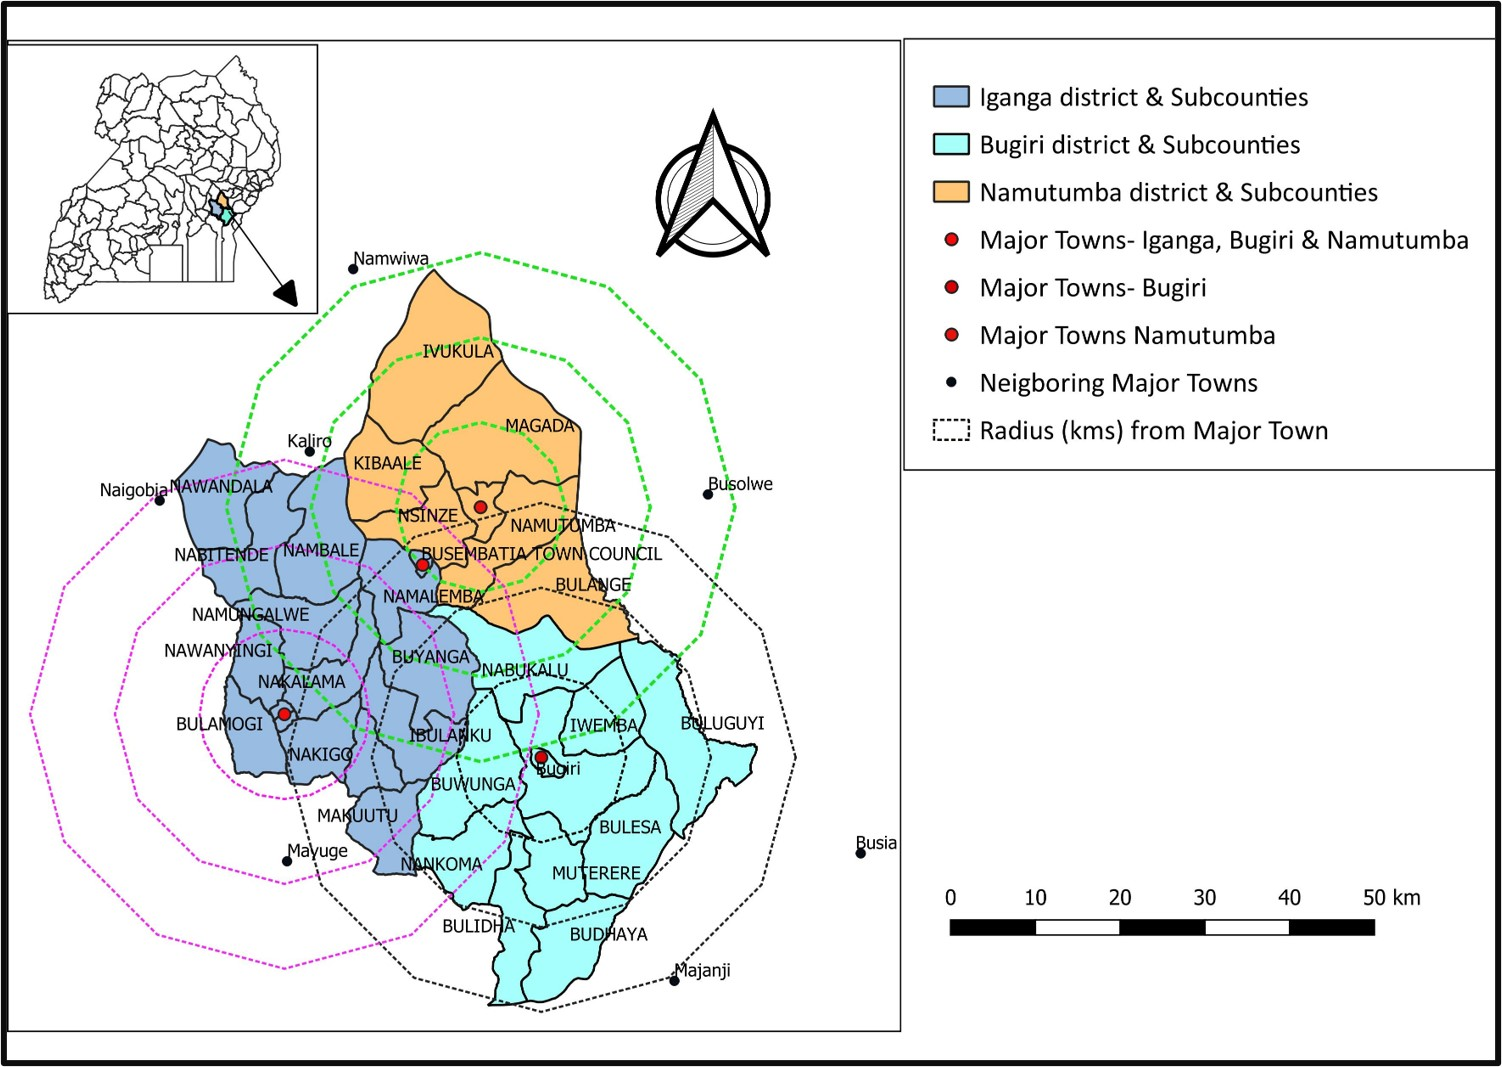
\includegraphics[scale=0.5]{map_outlined.jpg}\caption{Map of the study area.\label{fig:Map-of-the-study-area}}
\end{figure}

\begin{onehalfspace}
A key question that may arise is the degree to which results for the
three study districts can be generalized to Uganda as a whole. The
representativeness of the study area is examined using maize production
figures. The Eastern region, where the three districts fall, accounted
for the highest share (47\%) of the roughly 2.3 million tons of maize
harvested in 2009 \citep{Daly2016}. The district of Iganga was the
largest producer in the region and country, contributing 13.1\%, followed
by Mubende (7.4\%) in Central Uganda and Soroti (5.9\%) in Eastern
Uganda. The remaining districts contributed less than 4\%, including
Bugiri (2.7\%) which is part of this study.
\end{onehalfspace}

\newpage{}
\begin{onehalfspace}

\subsection{Variables\label{subsec:Variables} }
\end{onehalfspace}

\begin{onehalfspace}
The summary statistics for the main variables used in this study are
presented in tables~\ref{table:table1} and~\ref{table:table2}. Each
farmer rates a minimum of one input dealer, trader, or miller to a
maximum of three input dealers, traders, or millers (ratees). Farmer
perceptions about the ratees and ratee perceptions about themselves
are understood from the ratings given on four dimensions of location,
quality, price, and reputation. The averages of these dimension-based
ratings are obtained to get the overall average ratings (for both
farmer ratings and self-ratings). 

Several methods have been proposed and used to measure respondents\textquoteright{}
perceptions, attitudes, or beliefs in social science research. \citet{Delavande2011}
survey the literature on the measurement of subjective beliefs in
developing countries and categorize possible methods into three groups:
Likert style questions, elicitation of the \textquoteleft most likely\textquoteright{}
outcome, and a full elicitation of the distribution of beliefs, most
often conducted with visual aids. The ratings in this study reflect
Likert style assessment where the scores range from 1 to 5, 5 being
the best score and 1 being the worst score. This is the case for both
farmer ratings and self-ratings from the agro-input dealers, traders,
and millers\footnote{The farmer ratings are assumed to be not exposed to the input and
service providers before their self-ratings were collected.}. 
\end{onehalfspace}

Table~\ref{table:table1} presents the variables related to the farmers
in the dataset. The summary statistics for ratings based on all the
dimensions and the overall ratings are presented. Some interesting
trends are present in the ratings. For example, it is seen that about
6
percent of the farmers rated the ratees in the lowest category on
the location dimension (score of 1) while about 38
percent gave the highest rating for ease of reaching the ratee (score
of 5). Gender of the farmer is a dummy variable taking the value of
1 if the farmer is a woman and 0 otherwise. 

Gender based rating patterns indicate that female farmers are more
inclined to giving the highest score of 5 for location (41
percent) compared to male farmers (36
percent). Considering the dimensions, reputation and quality, larger
shares of male farmers give a rating of 5 compared to the female farmers.
Higher percentage of male farmers think that ease of access is poor
(at least level 2 score) and price competitiveness is poor (at least
level 2 score) while higher percentage of female farmers perceive
poorer reputation of the ratees (at least level 2 score). Same percentage
of male and female farmers perceive poor quality of services from
traders, millers, or input dealers.

Education and marital status are dummies indicating whether the farmer
has some level of education and whether the farmer is married. It
is interesting to note that 49
percent of the farmers are women, most of them have some level of
education (87
percent) and are married (86
percent). The average age of the farmers is 44.5.
The average distance of farmers' homestead to tarmac road is 6.54
kms and to murram road is 0.51
km. Dummy variable for interaction between farmers and the input dealer,
trader or processor is also included. 88
percent of the farmers have had some business interaction with the
individual they are rating. 

\begin{singlespace}
\begin{table} \footnotesize \begin{center} \begin{tabular}{@{\extracolsep{5pt}}lcccc}  \\[-1.8ex]\hline  \hline \\[-1.8ex]   & \multicolumn{4}{c}{\textit{Summary Statistics (Farmers)}} \\  
 \cline{2-5} \\[-1.8ex] & \multicolumn{1} {c} {Mean} &  \multicolumn{1} {c} {Standard Deviation} &  \multicolumn{1} {c} {Minimum} &  \multicolumn{1} {c} {Maximum} \\  
\hline \\[-1.8ex]  
{\textit{Overall rating (all ratees)}}                & $3.6$        & $0.77$        & $1$        & $5$ \\
{\textit{Location rating (all ratees)}}       & $3.88$        & $1.17$        & $1$        & $5$ \\
{\textit{Quality rating (all ratees)}}       & $3.5$        & $1.1$        & $1$        & $5$ \\
{\textit{Price rating (all ratees)}}       & $3.04$        & $1.08$        & $1$        & $5$ \\
{\textit{Reputation rating (all ratees)}}       & $3.83$        & $1.02$        & $1$        & $5$ \\
\hline \\[-1.8ex]  
{\textit{Overall rating (dealers)}}                & $3.59$        & $0.74$        & $1$        & $5$ \\
{\textit{Location rating (dealers)}}       & $3.65$        & $1.27$        & $1$        & $5$ \\
{\textit{Quality rating (dealers)}}       & $3.64$        & $1.02$        & $1$        & $5$ \\
{\textit{Price rating (dealers)}}       & $2.99$        & $1.08$        & $1$        & $5$ \\
{\textit{Reputation rating (dealers)}}       & $3.84$        & $0.96$        & $1$        & $5$ 
\\  
\hline \\[-1.8ex]  
{\textit{Overall rating (traders)}}                & $3.67$        & $0.8$        & $1$        & $5$ \\
{\textit{Location rating (traders)}}       & $4.09$        & $1.02$        & $1$        & $5$ \\
{\textit{Quality rating (traders)}}       & $3.54$        & $1.01$        & $1$        & $5$ \\
{\textit{Price rating (traders)}}       & $3.07$        & $1.05$        & $1$        & $5$ \\
{\textit{Reputation rating (traders)}}       & $3.84$        & $1.04$        & $1$        & $5$ 
\\  
\hline \\[-1.8ex]  
{\textit{Overall rating (millers)}}                & $3.54$        & $0.75$        & $1$        & $5$ \\
{\textit{Location rating (millers)}}       & $3.8$        & $1.21$        & $1$        & $5$ \\
{\textit{Quality rating (millers)}}       & $3.41$        & $1.19$        & $1$        & $5$ \\
{\textit{Price rating (millers)}}       & $3.02$        & $1.11$        & $1$        & $5$ \\
{\textit{Reputation rating (millers)}}       & $3.82$        & $1.03$        & $1$        & $5$ 
\\  
\hline \\[-1.8ex]  
{\textit{Gender}}       & $0.49$        & $0.5$        & $0$        & $1$ \\
{\textit{Age}}       & $44.5$        & $13.54$        & $16$        & $97$ \\
{\textit{Education}}       & $0.87$        & $0.34$        & $0$        & $1$ \\
{\textit{Marital Status}}       & $0.86$        & $0.34$        & $0$        & $1$ \\
{\textit{Distance of homestead to tarmac road}}       & $6.54$        & $7.7$        & $0$        & $90$ \\
{\textit{Distance of homestead to murram road}}       & $0.51$        & $1.17$        & $0$        & $15$ \\
{\textit{Interaction between farmers and all ratees}}       & $0.88$        & $0.33$        & $0$        & $1$ \\
{\textit{Interaction between farmers and dealers}}       & $0.8$        & $0.4$        & $0$        & $1$ \\
{\textit{Interaction between farmers and traders}}       & $0.84$        & $0.37$        & $0$        & $1$ \\
{\textit{Interaction between farmers and millers}}       & $0.95$        & $0.22$        & $0$        & $1$ 
\\ \hline   
 \end{tabular} \end{center}
\caption{Summary Statistics of the variables related to the farmers.} 
 \label{table:table1} 
 \end{table} 

\end{singlespace}

\begin{table} \footnotesize \begin{center} \begin{tabular}{@{\extracolsep{5pt}}lcccc}  \\[-1.8ex]\hline  \hline \\[-1.8ex]   & \multicolumn{4}{c}{\textit{Summary Statistics (Ratees)}} \\  
\cline{2-5} \\[-1.8ex] 
& \multicolumn{4} {c} {\textit{Agro-Input Dealers}}  \\
\cline{2-5} \\[-1.8ex]   
 & \multicolumn{1} {c} {Mean} &  \multicolumn{1} {c} {Standard Deviation} &  \multicolumn{1} {c} {Minimum} &  \multicolumn{1} {c} {Maximum} \\  
\hline \\[-1.8ex]  
{\textit{Overall self-ratings}}       & $4.13$        & $0.43$        & $2.8$        & $5$ \\
{\textit{Location self-ratings}}       & $4.22$        & $0.88$        & $2$        & $5$ \\
{\textit{Quality self-ratings}}       & $4.58$        & $0.61$        & $3$        & $5$ \\
{\textit{Price self-ratings}}       & $4.05$        & $0.82$        & $2$        & $5$ \\
{\textit{Reputation self-ratings}}       & $4.4$        & $0.86$        & $1$        & $5$ \\
{\textit{Gender}}       & $0.29$        & $0.46$        & $0$        & $1$ \\
{\textit{Age}}       & $35.95$        & $12.35$        & $19$        & $66$ \\
{\textit{Education}}       & $0.99$        & $0.11$        & $0$        & $1$ \\
{\textit{Marital Status}}       & $0.76$        & $0.43$        & $0$        & $1$ \\
\cline{2-5} \\[-1.8ex] 
& \multicolumn{4} {c} {\textit{Assembly Traders}}  \\
\cline{2-5} \\[-1.8ex]  
{\textit{Overall self-ratings}}       & $4.29$        & $0.5$        & $2.2$        & $5$ \\
{\textit{Location self-ratings}}       & $4.11$        & $0.85$        & $1$        & $5$ \\
{\textit{Quality self-ratings}}       & $4.33$        & $0.77$        & $1$        & $5$ \\
{\textit{Price self-ratings}}       & $3.91$        & $0.83$        & $1$        & $5$ \\
{\textit{Reputation self-ratings}}       & $4.45$        & $0.77$        & $2$        & $5$ \\
{\textit{Gender}}       & $0.02$        & $0.14$        & $0$        & $1$ \\
{\textit{Age}}       & $37.85$        & $9.56$        & $19$        & $80$ \\
{\textit{Education}}       & $0.96$        & $0.18$        & $0$        & $1$ \\
{\textit{Marital Status}}       & $0.96$        & $0.2$        & $0$        & $1$ \\
\cline{2-5} \\[-1.8ex] 
& \multicolumn{4} {c} {\textit{Millers}}  \\
\cline{2-5} \\[-1.8ex] 
{\textit{Overall self-ratings}}       & $4.18$        & $0.52$        & $3$        & $5$ \\
{\textit{Location self-ratings}}       & $3.99$        & $0.97$        & $1$        & $5$ \\
{\textit{Quality self-ratings}}       & $4.16$        & $0.84$        & $2$        & $5$ \\
{\textit{Price self-ratings}}       & $3.84$        & $0.95$        & $1$        & $5$ \\
{\textit{Reputation self-ratings}}       & $4.5$        & $0.69$        & $2$        & $5$ \\
{\textit{Gender}}       & $0.07$        & $0.25$        & $0$        & $1$ \\
{\textit{Age}}       & $36.68$        & $14.42$        & $17$        & $75$ \\
{\textit{Education}}       & $0.95$        & $0.21$        & $0$        & $1$ \\
{\textit{Marital Status}}       & $0.81$        & $0.39$        & $0$        & $1$
\\ \hline   
 \end{tabular} \end{center}
\caption{Summary Statistics of the variables related to the ratees (dealers, traders, and millers).} \label{table:table2} 
 \end{table} 

Table~\ref{table:table2} shows summary statistics for the self-ratings
from agro-input dealers, traders, and maize processors. The ratees
(dealers, traders, and millers) seem to be very confident about their
reputation as among all the dimensions, the highest percentage give
a self-score of 5 for reputation (58
percent). They seem to be the least confident about their location
as among all the dimensions, the highest percentage adhere to a score
of at least 2 for location. 

Gender, education, and marital status of these supply chain actors
are dummy variables. Women consist of 29
percent of the input dealers, only 2
percent of the traders and only 7
percent of the millers. A very good share of these supply chain actors
has some level of education and are married. Although the average
age of the dealers, traders and millers is between 35 and 40 years,
there is noticeable variation in the oldest actor observed. The oldest
input dealer is 66
years old; the oldest trader is 80
years old while the oldest miller is 75
years old. 

Looking at self-ratings based on the sex of the ratee, it is noticed
that among all the different dimensions, the greatest percentage of
female ratees rate themselves 5 for quality (68
percent) and the highest percentage of male ratees rate themselves
5 for reputation (59
percent). Giving self-scores of 5 is more common in women for location,
price, and quality. However, male ratees think themselves to be more
well reputed. Indeed, women think the quality of their services or
products are way better as they never rate themselves below 3 and
men think they are well reputed as only 1
percent of them rate themselves below 3. 

\begin{onehalfspace}
The primary variables of interest in this study are ratings (perceived
attributes) from farmers (raters), self-ratings (perceived self-attributes)
from ratees, the sex of the farmer and the ratee. In order to identify
the ratees as input dealers, traders or processors, unique identifiers
were attached to them. Similarly, unique identifiers were also assigned
to each farmer. 
\end{onehalfspace}
\begin{onehalfspace}

\subsection{Validity of ratings\label{subsec:Validity-of-ratings}}
\end{onehalfspace}

Testing whether the ratings are actually meaningful (instead of just
noise) is important. This will give better insights about the validity
of the perceptions. I look at intra-class correlation (ICC)\textbf{
}coefficients determining the level of agreement between the ratings.
In other words, ICC coefficients are a measure of inter or intra rater
reliability. Inter or intra rater reliability in the ratings literature
means levels of agreement between the ratings from different raters
\citep{gwet2014handbook}. Inter rater reliability (agreement) looks
at how close the ratings from different farmers are for an individual
ratee while intra rater reliability (agreement) looks at how close
the different ratings from an individual farmer are. 

\begin{onehalfspace}
Intra-class correlation coefficient can range between 0 and 1. The
lower it is, the poorer is the agreement and the higher it is, the
better is the agreement level. In this context, inter and intra-rater
reliability is studied for all the ratings given by the raters (farmers).
Only farmers who rated more than 6 times are considered for this analysis
(to reduce loss of observations during the analysis). The ICC coefficients
indicating inter-rater reliability compare the ratings for each ratee
from different farmers (raters). This helps to understand the level
of agreement among the farmers on the different attributes of a particular
ratee. The ICC coefficients indicating intra-rater reliability compare
the various ratings given by each individual farmer. This shows how
similar or different the farmer rates the various ratees. 

\begin{table} \small \begin{center} \begin{tabular}{@{\extracolsep{5pt}}lcc}  \\[-1.8ex]\hline  \hline \\[-1.8ex]   & \multicolumn{2}{c}{\textit{Intraclass correlation coefficients}} \\  
\cline{2-3} \\[-1.8ex] & \multicolumn{1} {c} {\textit{Inter-Rater Reliability}} &  \multicolumn{1} {c} {\textit{Intra-Rater Reliability}}  \\
  \hline \\[-1.8ex]  
{Overall}                 
&   $0.54$ 
&  $0.64$ 
\\
{Location}                
&   $0.47$ 
&  $0.62$ \\
{Quality}                 
&   $0.15$ 
&  $0.31$ \\
{Price}             
&   $0.43$ 
&  $0.43$ \\
{Reputation}                
&   $0.24$ 
&  $0.68$ 
 \\    \hline
 \end{tabular} \end{center}
\scriptsize
Note - The sample consists of all the raters and ratees (agro-input dealers, traders, and processors). The averaged overall ratings, ratings based on location, quality, price, and reputation are taken into account. ICC for Inter-Rater Reliability : Inter-rater reliability indicates the level of agreement between the ratings given by different individual farmer (rater) for the same ratee. The ratee being rated is constant during the comparison of the ratings. The sample consists of only the farmers who have rated more than 6 times. ICC for Intra-Rater Reliability : Intra-rater reliability focuses on the agreement between the different ratings given by each individual rater for different ratees. The farmer who has rated more than 6 times is constant during the comparison of the ratings. 
\caption{ICC coefficients for inter-rater reliability and intra-rater reliability.} \label{table:table3} 
 \end{table} 
\end{onehalfspace}

Table~\ref{table:table3} presents the ICC coefficients. Firstly,
it can be inferred that raters (farmers) agree decently on overall
ratings given to ratees. The ICC coefficient being 0.54,
it can be deduced that the ratings captured in the survey are not
entirely random or untrue. However, the level of agreement among the
raters (farmers) drops majorly for quality (0.15)
and reputation (0.24).
For location- and price-based ratings, the agreement levels are higher
(0.47,
0.43).
This is expected as location and prices are observable factors and
hence, ratings for these factors should be more similar compared to
non-observable attributes like quality and reputation. 

\begin{onehalfspace}
Secondly, analysing the overall averaged rating pattern, it can be
derived that every farmer rate in a similar way every dealer, trader
or miller. This is because the ICC coefficient is 0.64
(table~\ref{table:table3}), indicating a very decent level of agreement.
Similarly high levels of agreements are noticed for location (0.62)
and reputation (0.68)
based ratings. 

\newpage{}
\end{onehalfspace}
\begin{onehalfspace}

\section{Econometric Analysis\label{sec:Econometric-Analysis}}
\end{onehalfspace}

This section deals with the methodologies and estimation models used
for the analysis. In order to understand the rating patterns, mean
ratings from farmers and mean self-ratings are described in detail
in the next section. Ratings from farmers and self-ratings are compared
based on the sex of the farmers and the ratees, and differences in
how women rate other women and how men rate other men are presented
in section \ref{sec:Results}.

Next, I turn to the regression models to test the hypotheses laid
out in section \ref{sec:Study-Hypotheses}. In order to understand
gender-based impacts on the ratings from the farmers, the following
multivariate regression specification is used where the standard errors
are clustered at the ratee level:

\begin{singlespace}
\begin{equation} \label{eqn:eqn1} 
\begin{array}{l}
Y_{ija} = \beta_0 + \beta_1*Gender(F)_{ija} + \beta_2*Gender(R)_{ja} + \beta_3*X_{ija} + \\ &\quad \beta_4*Z_{ja} + \beta_5*\Gamma_{a} + e_{ija} 
\end{array}
\end{equation}
\end{singlespace}

Here, \emph{$Y_{ija}$} is the primary outcome variable, the ratings
from the farmers or the differences in ratings between the farmer
ratings and the self-ratings. The ratings are categorized into overall
average, location, quality, price, and reputation. In equation~\ref{eqn:eqn1},
\emph{i }is each individual farmer, \emph{j} is each individual ratee
and \emph{a} can be an agro-input dealer or assembly trader or processor
(ratee groups). The main independent variables are gender of the farmer
(\emph{$Gender(F)_{ija}$}, a dummy variable which takes the value
of 1 if the farmer is a woman and 0 otherwise) which can vary for
each individual farmer \emph{i}, each individual ratee \emph{j} and
each ratee group \emph{a} and the gender of the ratee (\emph{$Gender(R)_{ja}$},
a dummy variable taking the value of 1 for female ratee and 0 otherwise),
varying for each individual ratee \emph{j} and each ratee group \emph{a}.\emph{
$X_{ija}$} includes all the control variables varying for individual
farmer, ratee and ratee group. Those are age of the farmer, dummy
for interaction between the farmer and the ratee, dummy variable indicating
if the farmer has some level of education, distance of farmer's homestead
to tarmac and murram roads and marital status of farmer (dummy for
married farmers). \emph{$Z_{ja}$} consists of the control variables
varying for individual ratee and ratee group like age, education (dummy
for educated ratees) and dummy variable for marital status of the
ratee. The dummies for input dealer (takes the value of 1 if a dealer
and 0 otherwise) and trader (takes the value of 1 if a trader and
0 otherwise) are contained in \emph{$\Gamma_{a}$} where the ratee
being a miller is the reference category. The error term in the model
is \emph{$e_{ija}$}. The dataset used in the regression analyses
is pooled, i.e., ratings for dealers, traders and processors are contained
in the same dataset. 

Following this, for the analysis of how ratings vary if farmer (rater)
and ratee are of the same sex, an interaction term between the sex
of the farmer (rater) and the ratee (both dummy variables) is added
to the equation presented above. This is presented in the specification
below with cluster robust standard errors (equation~\ref{eqn:eqn2}):

\begin{onehalfspace}
\begin{equation} \label{eqn:eqn2} 
\begin{array}{l}
Y_{ija} = \beta_0 + \beta_1*Gender(F)_{ija} + \beta_2*Gender(R)_{ja} + \beta_3*X_{ija} + \beta_4*Z_{ja} + \\ &\quad \beta_5*\Gamma_{a} + \beta_6*Gender(F)_{ija}*Gender(R)_{ja} + e_{ija} 
\end{array}
\end{equation}
\end{onehalfspace}

The coefficients of interest in these models are\emph{ }$\beta_{1}$,
$\beta_{2}$ (equations~\ref{eqn:eqn1} and~\ref{eqn:eqn2}) and $\beta_{6}$
(equation~\ref{eqn:eqn2}), showing the gender impacts on the ratings
from farmers and the differences in farmer ratings and self-ratings. 

The final regression model aims to study the relationship between
the sex of the ratee and the self-ratings through multiple regression
analysis:

\begin{onehalfspace}
\begin{equation} \label{eqn:eqn3} 
\begin{array}{l}
Y_{ja} = \beta_0 + \beta_1*Gender(R)_{ja} + \beta_2*Z_{ja} + \beta_4*\Gamma_{a} + e_{ja} 
\end{array}
\end{equation}
\end{onehalfspace}

Here, the primary outcome variable of self-ratings is \emph{$Y_{ja}$,}
\emph{j} is each individual ratee and \emph{a} can be input dealer
or assembly trader or processor (ratee groups).\emph{ }$\beta_{1}$
indicates the relationship between the sex of the ratee and the self-rating
from the ratee. Some of the variables discussed above are included
in this equation. The main independent variable is gender of the ratee
(\emph{$Gender(R)_{ja}$}). \emph{$Z_{ja}$ }and \emph{$\Gamma_{a}$}
consists of the control variables and the dummies for input dealer
and trader. The error term in this model is \emph{$e_{ja}$}. 

An essential discussion is the motivation behind the inclusion of
the control variables discussed in the models above. Men are likely
to be better educated than women. Better levels of education and knowledge
will probably mean that farmers have a better understanding of what
to expect from service and input providers, and so, may rate more
or less favourably (the ratings or scores given will be better informed).
One does have to control for this impact pathway as otherwise, the
gender and education effects will be conflated. In other words, correlation
between the farmer's gender and the rating from the farmer may be
confounded by education. Women are likely to be younger than men because
of recent entry into farming activities and, older women devote more
time to family responsibilities. Thus, age may directly affect ratings.
For instance, older individuals may have more experience and so, may
rate more or less critically. Therefore, age effects need to be purged
from the model by controlling for it. Like age, mobility may directly
affect ratings. In particular, men are more mobile and so more likely
to have interacted with input dealers. If these interactions lead
to systematically different ratings, it is necessary to control for
it. 

Distance to murram and tarmac roads are proxies of remoteness. In
remote areas, input and service providers face many challenges such
as larger transaction costs and poor access to services such as power.
For instance, in semi-urban areas, mills often run on 3-phase electricity,
while in remote areas, combustion engines are used to power the mills.
The latter produce inferior quality maize products. These differences
will be reflected in the ratings because farmers in remote areas tend
to reach out to the input and service providers operating in those
same areas. Thus, by controlling for distance of farmer's homestead
to murram and tarmac roads, these differences are accounted for.

Men in farming activities tend to be married. On the other hand, it
can be expected that women in farming are mostly not married as married
women get involved more in household activities. Being married could
mean that these farmers have been longer in maize production and thus,
have more experience with service and input providers. This might
make their ratings more or less favourable which makes it important
to control for marital status of the farmer. 

The arguments can be similar in the case of ratees. Since men are
likely to be more educated than women, the education and knowledge
might define what kind of service and inputs they provide to their
customers (better or worse knowledge of improved services or inputs).
This would lead to more or less favourable ratings from farmers and
self-ratings, justifying the need to control for education of ratees.
Men are likely to be older because of longer active periods in service
providing and input dealing. Older individuals might have better experience
in the business. This can impact the ratings. Farmers may rate older
ratees with more experience more favourably while self-ratings are
likely to be higher from older individuals because of their greater
awareness about their performance in the sector. Hence, I control
for age of the ratee (input dealer, trader, or miller). 

Controlling for marital status of ratees is necessary as married service
and input providers mostly tend to be men. This would mean they would
have better knowledge and experience (more time spent in business
as the chances of being married increases with age) which might lead
to more favourable ratings from farmers. At the same time, women who
are not married might be rating themselves lower because of minimal
experience, knowledge, connections, and support in their businesses.
Therefore, purging marital status effects of the ratees from the model
is essential. 

\begin{onehalfspace}
\newpage{}
\end{onehalfspace}
\begin{onehalfspace}

\section{Results\label{sec:Results} }
\end{onehalfspace}

This section focuses on the results obtained from the analysis of
average ratings from farmers and average self-ratings given by ratees
to themselves. Furthermore, the regression results are  presented
and discussed below. 
\begin{onehalfspace}

\subsection{Average ratings\label{subsec:Average-ratings}}
\end{onehalfspace}

\begin{onehalfspace}
Average scores are obtained for the ratings given by the farmers (raters)
to the ratees (agro-input dealers, processors, and traders) and for
the self-ratings by the ratees themselves. The primary goal of this
section is to check whether the mean ratings obtained from the dataset
(presented in table~\ref{table:table4}) reiterate the hypotheses
of the study\footnote{The results for traders and millers may suffer from small sample share
of women.}. 

\begin{landscape}
\begin{table}
\footnotesize \begin{center} \begin{tabular}{@{\extracolsep{5pt}}lcccccccccccc}  \\[-1.8ex]\hline  \hline \\[-1.8ex]   & \multicolumn{12}{c}{\textit{Average Ratings (Mean)}} \\  
\cline{2-13} \\[-1.8ex] 
& \multicolumn{12} {c} {\textit{Overall Average (All Dimensions)}}  \\
\cline{2-13} \\[-1.8ex]   & \multicolumn{3} {c} {All Ratees} &  \multicolumn{3} {c} {Agro-Input Dealers} &  \multicolumn{3} {c} {Assembly Traders} &  \multicolumn{3} {c} {Millers} \\  
 & \multicolumn{1} {c} {\textit{Men}} &  \multicolumn{1} {c} {\textit{Women}} &  \multicolumn{1} {c} {\textit{All}} &  \multicolumn{1} {c} {\textit{Men}} &  \multicolumn{1} {c} {\textit{Women}} &  \multicolumn{1} {c} {\textit{All}} &  \multicolumn{1} {c} {\textit{Men}} &  \multicolumn{1} {c} {\textit{Women}} &  \multicolumn{1} {c} {\textit{All}} &  \multicolumn{1} {c} {\textit{Men}}  &  \multicolumn{1} {c} {\textit{Women}} &  \multicolumn{1} {c} {\textit{All}} \\
\hline \\[-1.8ex]  
{\textit{Male farmers}}                & $3.58$ 
&  $3.61$
&  $3.58$
&  $3.59$
&  $3.57$
&  $3.58$
&  $3.64$
&  $3.92$
&  $3.65$
&  $3.51$
&  $3.59$
&  $3.52$
\\
{\textit{Female farmers}}        & $3.62$ 
&  $3.63$
&  $3.62$
&  $3.6$
&  $3.64$
&  $3.61$
&  $3.68$
&  $4.09$
&  $3.69$
&  $3.58$
&  $3.44$
&  $3.57$       \\
{\textit{All farmers}}         & $3.59$ 
&  $3.61$
&  $3.6$
&  $3.59$
&  $3.59$
&  $3.59$
&  $3.66$
&  $4$
&  $3.66$
&  $3.54$
&  $3.53$
&  $3.54$       \\
{\textit{Self-ratings}}            & $4.23$ 
&  $4.16$
&  $4.22$
&  $4.06$
&  $4.02$
&  $4.05$
&  $4.28$
&  $4.53$
&  $4.28$
&  $4.23$
&  $4.29$
&  $4.24$       \\

\cline{2-13} \\[-1.8ex] 
& \multicolumn{12} {c} {\textit{Location}}  \\
\cline{2-13} \\[-1.8ex]  
{\textit{Male farmers}}                & $3.85$ 
&  $3.54$
&  $3.83$
&  $3.61$
&  $3.33$
&  $3.53$
&  $4.05$
&  $4.41$
&  $4.06$
&  $3.76$
&  $3.74$
&  $3.76$
\\
{\textit{Female farmers}}        & $3.98$ 
&  $3.82$
&  $3.97$
&  $3.93$
&  $3.77$
&  $3.89$
&  $4.13$
&  $4.4$
&  $4.13$
&  $3.87$
&  $3.67$
&  $3.86$       \\
{\textit{All farmers}}         & $3.91$ 
&  $3.64$
&  $3.88$
&  $3.72$
&  $3.46$
&  $3.65$
&  $4.08$
&  $4.41$
&  $4.09$
&  $3.81$
&  $3.71$
&  $3.8$       \\
{\textit{Self-ratings}}            & $4.11$ 
&  $4.07$
&  $4.11$
&  $4.08$
&  $4.01$
&  $4.06$
&  $4.1$
&  $4.97$
&  $4.12$
&  $4.12$
&  $3.91$
&  $4.11$       \\

\cline{2-13} \\[-1.8ex] 
& \multicolumn{12} {c} {\textit{Quality}}  \\
\cline{2-13} \\[-1.8ex]  

{\textit{Male farmers}}                & $3.49$ 
&  $3.7$
&  $3.51$
&  $3.71$
&  $3.65$
&  $3.69$
&  $3.53$
&  $3.82$
&  $3.54$
&  $3.37$
&  $3.77$
&  $3.39$
\\
{\textit{Female farmers}}        & $3.47$ 
&  $3.65$
&  $3.49$
&  $3.48$
&  $3.64$
&  $3.52$
&  $3.54$
&  $3.93$
&  $3.55$
&  $3.41$
&  $3.56$
&  $3.42$       \\
{\textit{All farmers}}         & $3.48$ 
&  $3.68$
&  $3.5$
&  $3.63$
&  $3.65$
&  $3.64$
&  $3.53$
&  $3.88$
&  $3.54$
&  $3.39$
&  $3.69$
&  $3.41$       \\
{\textit{Self-ratings}}            & $4.24$ 
&  $4.68$
&  $4.28$
&  $4.48$
&  $4.62$
&  $4.52$
&  $4.3$
&  $4.88$
&  $4.31$
&  $4.12$
&  $4.71$
&  $4.16$       \\

\cline{2-13} \\[-1.8ex] 
& \multicolumn{12} {c} {\textit{Price}}  \\
\cline{2-13} \\[-1.8ex]  

{\textit{Male farmers}}                & $3.01$ 
&  $2.95$
&  $3$
&  $2.96$
&  $2.92$
&  $2.95$
&  $3.05$
&  $3.24$
&  $3.05$
&  $2.99$
&  $2.93$
&  $2.98$
\\
{\textit{Female farmers}}        & $3.1$ 
&  $3$
&  $3.09$
&  $3.08$
&  $3.09$
&  $3.08$
&  $3.09$
&  $3.47$
&  $3.1$
&  $3.1$
&  $2.69$
&  $3.08$       \\
{\textit{All farmers}}         & $3.04$ 
&  $2.97$
&  $3.04$
&  $3$
&  $2.97$
&  $2.99$
&  $3.07$
&  $3.34$
&  $3.07$
&  $3.04$
&  $2.83$
&  $3.02$       \\
{\textit{Self-ratings}}            & $3.9$ 
&  $4.06$
&  $3.92$
&  $3.82$
&  $4.05$
&  $3.88$
&  $3.93$
&  $3.94$
&  $3.93$
&  $3.91$
&  $4.14$
&  $3.92$       \\

\cline{2-13} \\[-1.8ex] 
& \multicolumn{12} {c} {\textit{Reputation}}  \\
\cline{2-13} \\[-1.8ex]  
{\textit{Male farmers}}                & $3.82$ 
&  $3.93$
&  $3.83$
&  $3.82$
&  $3.96$
&  $3.86$
&  $3.81$
&  $4.06$
&  $3.82$
&  $3.83$
&  $3.84$
&  $3.83$
\\
{\textit{Female farmers}}        & $3.83$ 
&  $3.93$
&  $3.84$
&  $3.78$
&  $3.89$
&  $3.81$
&  $3.85$
&  $4.4$
&  $3.87$
&  $3.82$
&  $3.79$
&  $3.82$       \\
{\textit{All farmers}}         & $3.82$ 
&  $3.93$
&  $3.83$
&  $3.81$
&  $3.94$
&  $3.84$
&  $3.83$
&  $4.22$
&  $3.84$
&  $3.83$
&  $3.82$
&  $3.82$       \\
{\textit{Self-ratings}}            & $4.48$ 
&  $4.34$
&  $4.47$
&  $4.53$
&  $4.4$
&  $4.49$
&  $4.38$
&  $4$
&  $4.37$
&  $4.55$
&  $4.33$
&  $4.54$      
\\ \hline   
 \end{tabular} \end{center}
\caption{Average ratings (all dimensions) from farmers and average self-ratings (all dimensions) from dealers, traders, and processors, grouped by gender.} 
\label{table:table4} 
 \end{table}
\end{landscape}Table~\ref{table:table4} shows that the mean overall self-rating
given by the ratees (4.22)
is higher than the mean rating from the farmers (3.6).
This phenomenon is consistent across all the different rating dimensions.
Looking at individual groups of input dealers, traders, and millers
in table~\ref{table:table4}, the same inference can be made that
self-ratings are always higher. These findings support hypothesis
\ref{Hypothesis 1}. 

In order to validate hypothesis \ref{Hypothesis 2} from the trends
in the dataset, I will first look at the entire group of ratees. The
mean overall rating from female farmers is 3.62
which is higher than the mean overall rating given by male farmers
(3.58).
Similar pattern is noticed for location-, price- and reputation-based
ratings. However, for quality-based rating, male farmers give a higher
rating. Interestingly, these patterns vary across the groups of input
dealers, traders, and millers. For overall average ratings, location-
and price-based ratings, female farmers always give better scores
to dealers, traders and processors. Male farmers give better scores
for quality to dealers while lower scores for quality to traders and
millers when compared to their female counterparts. More favourable
scores for reputation of dealers and millers come from men while for
traders, come from women. Thus, hypothesis \ref{Hypothesis 2} is
generally true with an exception for quality- and reputation-based
ratings from the farmers. 
\end{onehalfspace}

Next, I focus on the comparison of self-ratings from women and men.
For overall average self-rating, women (4.16)
rate lower compared to men (4.23).
This is consistent for location and reputation based self-ratings.
However, for quality and price, men self-assess themselves worse than
how women self-assess themselves. These findings are similar for each
rating dimension in the case of input dealers. Self-ratings from male
assembly traders are always lower than female assembly traders except
when they are rating for reputation. The results obtained from the
mean self-ratings of the entire ratee group reflect in the results
for the miller group in particular. However, the only exception is
the overall average self-rating where male millers assess themselves
worse than the female millers. Thus, supporting hypothesis \ref{Hypothesis 3},
it can be stated that although women tend to generally self-assess
less favourably; for quality and price, women tend to self-assess
more favourably when compared to men.

Following this, the focus is on the sex of the ratees and the ratings
from the farmers. Men receive less favourable ratings for overall
average, quality, and reputation. For location and price, women receive
better scores than men. These findings are consistent for the group
of agro-input dealers across the rating dimensions. However, both
male and female input dealers receive the same overall average rating.
Interestingly, all male assembly traders receive lower scores across
all the rating dimensions than the female assembly traders. Thus,
female assembly traders are perceived to be performing better. In
the case of millers, women always receive less favourable ratings,
with an exception for quality. Thus, hypothesis \ref{Hypothesis 4}
does not entirely align with these findings from table~\ref{table:table4}.
Women mostly are rated lower for location and price whereas men are
rated worse overall and for quality and reputation mostly. 

Next, I examine how men rate other men and women rate other women.
The average ratings show that women give more favourable ratings to
other women compared to men's ratings for other men, only in the case
of overall average, quality, and reputation. All female traders are
always rated higher by female farmers in every dimension of rating.
Male millers are generally rated higher by male farmers with an exception
for quality. Women rate female agro-input dealers higher for all aspects
except for quality. These findings portray the underlying idea of
hypothesis \ref{Hypothesis 5}.

It is interesting to note that generally, women are always rated higher
for quality (consistent for dealers, traders, and processors), indicating
provision of better quality from women. Similarly, men are consistently
rated higher for location with an exception for traders. This may
indicate that women (dealers and millers) are located in poorer locations.
Some of the reasons behind that could be mobility constraints, lack
of capital to set up businesses in better locations and less knowledge
of good locations for business. 

Farmer ratings indicate that price competitiveness of male input dealers
and millers are perceived to be better, women in input dealing and
trading and men in processing of maize are perceived to be well-reputed.
The rating attribute that is always scored the lowest is price competitiveness
and that is always scored the highest is ease of access for traders
and reputation for agro-input dealers and millers. Input dealers get
the lowest score for ease of access and price competitiveness and
millers get the lowest rating for overall average, quality, and reputation.
Thus, agro-input dealers are overall not easy to reach while assembly
traders are. In terms of the quality of service provided, input dealers
are perceived to be the best in comparison to traders and millers. 
\begin{onehalfspace}

\subsection{Regressions\label{subsec:Regressions}}
\end{onehalfspace}

Tables~\ref{table:table5},~\ref{table:table6} and~\ref{table:table7}
present results from the regressions implemented for this study. Table~\ref{table:table5}
shows multivariate regressions with clustered standard errors (at
the ratee level), discussing the impact of the sex of the farmer (rater)
and the ratee on the ratings given by the farmers to the ratees. From
model 1, it is noticeable that the impact of the sex of the farmer
on the average overall rating given by the farmer is significant.
If the farmer is a woman, the average score given by the farmer is
0.06
higher. Thus, female farmers give more favourable ratings when compared
to male farmers, consistent with the results from table~\ref{table:table4}.
The relation between the gender of the ratee (dealer, trader, or miller)
and the overall average ratings given by the farmer is insignificant. 

\begin{onehalfspace}
If the farmer had some business interaction with the input dealer,
trader, or processor the farmer is rating, the rating given by the
farmer is approximately 0.4
point higher (significant). The education level of the farmer significantly
influences the way the farmer rates the ratee. If the farmer has some
level of education, the farmer (rater) rates the ratee 0.09
point higher. The negative relation between the average overall rating
given by the farmer and the distance of the farmer's homestead from
the nearest murram road is also significant. This means greater distance
from the murram road would imply a lower score given by the farmer
(rater). There is a negative relationship between the ratee's marital
status, and the ratings received by the ratee. If the ratee is married,
the ratee receives a significantly lower score. Ratings for dealers
are higher on average by approximately 0.09
point (significant) and ratings for traders are significantly higher
on average by 0.19
point (consistent with table~\ref{table:table4} results). The total
number of observations is 3589. 
\end{onehalfspace}

The interaction between the sex of the farmer and the sex of the ratee
is insignificant throughout all the models in table~\ref{table:table5}.
In other words, no significant gender based homophily effect is found
(disproving hypothesis \ref{Hypothesis 5}). The positive relationship
between sex of the farmer and the farmer's ratings is significantly
consistent for location-based and price-based ratings (models 3, 4,
7 and 8). This is consistent with the results from table~\ref{table:table4}.
However, the magnitude of more favourable ratings from female farmers
is most noticeable for location-based ratings, being highly significant
too. Interestingly, for quality- and reputation-based ratings, if
the ratee is a woman, the farmer's rating increases significantly.
However, the ratings decline for location-based ratings if the ratee
is a woman (similar findings in table~\ref{table:table4}). Thus,
it can be inferred that female farmers give more favourable scores
overall (proving hypothesis \ref{Hypothesis 2}), particularly for
location and price and female ratees receive better scores from farmers
only for quality and reputation (disproving hypothesis \ref{Hypothesis 4}). 

\begin{onehalfspace}
\begin{landscape}
\begin{table} \scriptsize \begin{center} \begin{tabular}{@{\extracolsep{5pt}}lcccccccccc}  \\[-1.8ex]\hline  \hline \\[-1.8ex]   & \multicolumn{10}{c}{\textit{\footnotesize Dependent variable: Ratings from Farmers (Raters)}} \\  
\cline{2-11} \\[-1.8ex] & \multicolumn{2} {c} {\scriptsize Overall} &  \multicolumn{2} {c} {\scriptsize Location}  &
\multicolumn{2} {c} {\scriptsize Quality}&
\multicolumn{2} {c} {\scriptsize Price}&
\multicolumn{2} {c} {\scriptsize Reputation} \\
\\[-1.8ex] & (\scriptsize 1) & (\scriptsize 2) & (\scriptsize 3) & (\scriptsize 4) & (\scriptsize 5)& (\scriptsize 6) & (\scriptsize 7) & (\scriptsize 8) & (\scriptsize 9) & (\scriptsize 10) \\  \hline \\[-1.8ex]  
{Intercept}                  & $3.0954^{***}$ 
& $3.095^{***}$ 
 & $3.5511^{***}$ 
& $3.554^{***}$ 
 & $2.6314^{***}$   
      & $2.6314^{***}$ 
& $2.9595^{***}$ 
 & $2.9584^{***}$ 
& $3.3677^{***}$ 
 & $3.3673^{***}$ 
\\                              & $(0.1649)$     & $(0.1648)$   & $(0.2925)$     & $(0.292)$     & $(0.2817)$ 
             & $(0.2816)$     & $(0.2014)$   & $(0.2013)$     & $(0.1876)$     & $(0.1876)$      
\\ {Gender(F)}
& $0.062^{**}$ 
& $0.0635^{**}$ 
 & $0.1499^{***}$ 
& $0.1381^{***}$ 
 & $0.0087^{}$   
      & $0.0087^{}$ 
& $0.09^{**}$ 
 & $0.0944^{**}$ 
& $0.0074^{}$ 
 & $0.0091^{}$ 
\\                              & $(0.0293)$     & $(0.0306)$   & $(0.0485)$     & $(0.0505)$     & $(0.0429)$ 
             & $(0.0446)$     & $(0.0408)$   & $(0.0426)$     & $(0.0373)$     & $(0.0388)$   
\\ {Gender(R)}  
               & $0.0418^{}$ 
& $0.0487^{}$ 
 & $-0.1205^{}$ 
& $-0.1753^{*}$ 
 & $0.1733^{**}$   
      & $0.1734^{**}$ 
& $-0.0549^{}$ 
 & $-0.0341^{}$ 
& $0.1232^{*}$ 
 & $0.1308^{}$ 
\\                              & $(0.0721)$     & $(0.0725)$   & $(0.1306)$     & $(0.1414)$     & $(0.1073)$ 
             & $(0.1081)$     & $(0.0886)$   & $(0.0853)$     & $(0.0778)$     & $(0.0934)$            
\\ {Age of farmer}
               & $0.0011^{}$ 
& $0.0949^{**}$ 
 & $0.0021^{}$ 
& $0.1298^{**}$ 
 & $0.0003^{}$   
      & $0.1132^{*}$ 
& $0.0011^{}$ 
 & $0.1334^{**}$ 
& $0^{}$ 
 & $0.0076^{}$ 
\\                              & $(0.0012)$     & $(0.0437)$   & $(0.0018)$     & $(0.0686)$     & $(0.0016)$ 
             & $(0.0608)$     & $(0.0016)$   & $(0.0614)$     & $(0.0014)$     & $(0.0519)$            
\\ {Interaction}                & $0.3985^{***}$ 
& $0.3985^{***}$ 
 & $0.251^{***}$ 
& $0.2509^{***}$ 
 & $0.4942^{***}$   
      & $0.4942^{***}$ 
& $0.2348^{***}$ 
 & $0.2349^{***}$ 
& $0.4333^{***}$ 
 & $0.4333^{***}$ 
\\                              & $(0.0468)$     & $(0.0468)$   & $(0.0648)$     & $(0.0648)$     & $(0.0589)$ 
             & $(0.0589)$     & $(0.0552)$   & $(0.0552)$     & $(0.0557)$     & $(0.0557)$            
\\ {Education(F)}
               & $0.0947^{**}$ 
& $0.0011^{}$ 
 & $0.131^{**}$ 
& $0.0021^{}$ 
 & $0.1132^{*}$   
      & $0.0003^{}$ 
& $0.133^{**}$ 
 & $0.0011^{}$ 
& $0.0074^{}$ 
 & $0^{}$ 
\\                              & $(0.0437)$     & $(0.0012)$   & $(0.0684)$     & $(0.0018)$     & $(0.0608)$ 
             & $(0.0016)$     & $(0.0613)$   & $(0.0016)$     & $(0.0519)$     & $(0.0014)$            
\\   {Tarmac}
               & $-0.0023^{}$ 
& $-0.0023^{}$ 
 & $-0.0015^{}$ 
& $-0.0015^{}$ 
 & $-0.0067^{***}$   
      & $-0.0067^{***}$ 
& $-0.0046^{**}$ 
 & $-0.0046^{**}$ 
& $0.0014^{}$ 
 & $0.0015^{}$ 
\\                              & $(0.0022)$     & $(0.0022)$   & $(0.0039)$     & $(0.0039)$     & $(0.0032)$ 
             & $(0.0032)$     & $(0.0026)$   & $(0.0026)$     & $(0.0026)$     & $(0.0026)$            
\\  {Murram}
               & $-0.0191^{*}$ 
& $-0.0191^{*}$ 
 & $-0.0286^{*}$ 
& $-0.0288^{*}$ 
 & $-0.0084^{}$   
      & $-0.0084^{}$ 
& $-0.0141^{}$ 
 & $-0.014^{}$ 
& $0.0018^{}$ 
 & $0.0019^{}$ 
\\                              & $(0.0094)$     & $(0.0094)$   & $(0.0171)$     & $(0.0171)$     & $(0.0141)$ 
             & $(0.0141)$     & $(0.0129)$   & $(0.0129)$     & $(0.0125)$     & $(0.0125)$            
\\    {Farmer marital status}
               & $-0.063^{}$ 
& $-0.0631^{}$ 
 & $-0.0675^{}$ 
& $-0.0666^{}$ 
 & $-0.0344^{}$   
      & $-0.0344^{}$ 
& $-0.0913^{}$ 
 & $-0.0917^{}$ 
& $-0.0834^{}$ 
 & $-0.0835^{}$ 
\\                              & $(0.0445)$     & $(0.0445)$   & $(0.0732)$     & $(0.0733)$     & $(0.061)$ 
             & $(0.061)$     & $(0.0662)$   & $(0.0663)$     & $(0.0547)$     & $(0.0547)$            
\\   {Age of ratee}
               & $0.0018^{}$ 
& $0.0018^{}$ 
 & $0.0009^{}$ 
& $0.0009^{}$ 
 & $0.0044^{***}$   
      & $0.0044^{***}$ 
& $0.0007^{}$ 
 & $0.0007^{}$ 
& $0.0026^{*}$ 
 & $0.0026^{*}$ 
\\                              & $(0.0017)$     & $(0.0017)$   & $(0.0026)$     & $(0.0026)$     & $(0.0032)$ 
             & $(0.0032)$     & $(0.0022)$   & $(0.0023)$     & $(0.0021)$     & $(0.0021)$            
\\ {Ratee marital status} 
               & $-0.1142^{***}$ 
& $-0.114^{***}$ 
 & $-0.1244^{*}$ 
& $-0.1255^{*}$ 
 & $-0.1591^{***}$   
      & $-0.1591^{***}$ 
& $-0.1283^{**}$ 
 & $-0.1279^{**}$ 
& $-0.081^{}$ 
 & $-0.0809^{}$ 
\\                              & $(0.0565)$     & $(0.0565)$   & $(0.107)$     & $(0.1066)$     & $(0.1045)$ 
             & $(0.1046)$     & $(0.0708)$   & $(0.0708)$     & $(0.0641)$     & $(0.0643)$            
\\ {Education(R)}
               & $0.0138^{}$ 
& $0.0135^{}$ 
 & $-0.0968^{}$ 
& $-0.0952^{}$ 
 & $0.2425^{**}$   
      & $0.2425^{**}$ 
& $-0.1613^{}$ 
 & $-0.162^{}$ 
& $0.0663^{}$ 
 & $0.0661^{}$ 
\\                              & $(0.1145)$     & $(0.1147)$   & $(0.1778)$     & $(0.1761)$     & $(0.22)$ 
             & $(0.2201)$     & $(0.1032)$   & $(0.1028)$     & $(0.1368)$     & $(0.1368)$            
\\ {Dealer dummy} 
               & $0.0888^{**}$ 
& $0.0887^{**}$ 
 & $-0.0919^{}$ 
& $-0.0908^{}$ 
 & $0.2256^{***}$   
      & $0.2256^{***}$ 
& $0.0066^{}$ 
 & $0.0061^{}$ 
& $0.0403^{}$ 
 & $0.0401^{}$ 
\\                              & $(0.0452)$     & $(0.0451)$   & $(0.1068)$     & $(0.1067)$     & $(0.0838)$ 
             & $(0.0838)$     & $(0.0646)$   & $(0.0646)$     & $(0.0531)$     & $(0.053)$  
\\ {Trader dummy} 
                       & $0.1908^{***}$ 
& $0.1908^{***}$ 
 & $0.3321^{***}$ 
& $0.3322^{***}$ 
 & $0.2195^{***}$   
      & $0.2195^{***}$ 
& $0.0966^{**}$ 
 & $0.0965^{**}$ 
& $0.0734^{*}$ 
 & $0.0734^{*}$ 
\\                              & $(0.0414)$     & $(0.0414)$   & $(0.0653)$     & $(0.0653)$     & $(0.0755)$ 
             & $(0.0755)$     & $(0.0529)$   & $(0.0529)$     & $(0.0505)$     & $(0.0505)$            
\\ {Gender(F):Gender(R)} 
               & 
& $-0.0187^{}$ 
 & 
& $0.1482^{}$ 
 &    
      & $-0.0005^{}$ 
& 
 & $-0.0563^{}$ 
& 
 & $-0.0207^{}$ 
\\                              &     & $(0.086)$   &      & $(0.167)$     & 
             & $(0.1248)$     &    & $(0.1221)$     &    & $(0.1207)$          
    \\ \hline 
R$^2$                   & $0.0408$       & $0.0408$       & $0.0341$       & $0.0344$    & $0.0374$ & $0.0374$ & $0.0136$ & $0.0137$ & $0.0212$ & $0.0212$ 
 \\ Adj. R$^2$                         & $0.0373$       & $0.0371$       & $0.0306$       & $0.0306$    & $0.0339$ & $0.0336$ & $0.01$ & $0.0098$ & $0.0177$ & $0.0174$ 
\\ Number of obs.                     & $3589$       & $3589$       & $3589$       & $3589$    & $3589$ & $3589$ & $3589$ & $3589$ & $3589$ & $3589$ 
     \\ \hline
\multicolumn{10}{l}{ \tiny{$^{***}p<0.01$; $^{**}p<0.05$; $^{*}p<0.1$.}} 
 \end{tabular} \end{center}
\tiny
Note: Standard errors are clustered at the ratee level (agro-input dealers, traders, and millers). The dependent variable is the rating given by the farmers and the main independent variables are farmer's and ratee's gender. The dimensions based on which the ratings are given are overall average (models 1, 2), location (models 3, 4), quality (models 5, 6), price (models 7, 8) and reputation (models 9, 10). Models 2, 4, 6, 8 and 10 include an interaction between the farmer's and ratee's gender while the other models do not. F refers to farmers and R refers to ratees. 
\caption{Regression results for the impact of farmer's (rater's) and ratee's gender on the ratings given by the farmers to the ratees.} \label{table:table5} 
 \end{table} \end{landscape}
\end{onehalfspace}

Following this, table~\ref{table:table6} shows the results from multiple
regression analysis looking at the impact of sex of the ratee on self-assessments
(self-ratings). The relationship is significant only for quality-,
price- and reputation-based self-ratings. If the ratee is a woman,
she significantly self-assesses herself higher than the male ratees
for quality and price. However, for reputation, she rates herself
lower (significant). These results are consistent with the findings
from table~\ref{table:table4}. Looking at model 1, it can be noted
that older and educated ratees self-assess themselves higher significantly
and married ratees self-assess themselves lower significantly. Consistent
with table~\ref{table:table4} results, it can be observed that traders
significantly give higher self-ratings while dealers give significantly
lower self-ratings. Henceforth, it can be inferred that for quality
and price, women self-assess themselves higher while for reputation,
lower. Here, hypothesis \ref{Hypothesis 3} is only consistent with
the finding about reputation based self-ratings. 

\begin{onehalfspace}
\begin{table} \small \begin{center} \begin{tabular}{@{\extracolsep{5pt}}lccccc}  \\[-1.8ex]\hline  \hline \\[-1.8ex]   & \multicolumn{5}{c}{\textit{Dependent variable: Self-ratings by dealers, traders, and millers}} \\  
\cline{2-6} \\[-1.8ex] & \multicolumn{1} {c} {Overall} &  \multicolumn{1} {c} {Location}  &
\multicolumn{1} {c} {Quality}&
\multicolumn{1} {c} {Price}&
\multicolumn{1} {c} {Reputation} \\
\\[-1.8ex] & (1) & (2) & (3) & (4) & (5) \\  \hline \\[-1.8ex]  
{Intercept}                  & $4.0737^{***}$ 
& $3.896^{***}$ 
 & $3.9657^{***}$ 
& $3.438^{***}$ 
 & $4.7091^{***}$   
\\                              & $(0.053)$     & $(0.1035)$   & $(0.086)$     & $(0.0958)$     & $(0.0798)$ 
                    
\\ {Gender(R)}  
              & $0.0353^{}$ 
& $-0.0289^{}$ 
 & $0.391^{***}$ 
& $0.2388^{***}$ 
 & $-0.197^{***}$   
\\                              & $(0.0301)$     & $(0.0588)$   & $(0.0489)$     & $(0.0544)$     & $(0.0454)$     
           
\\   {Age of ratee}
                 & $0.0021^{***}$ 
& $0.0064^{***}$ 
 & $-0.0013^{}$ 
& $0.0084^{***}$ 
 & $0.001^{}$   
\\                              & $(0.0007)$     & $(0.0014)$   & $(0.0012)$     & $(0.0013)$     & $(0.0011)$

\\ {Ratee marital status} 
                & $-0.0575^{**}$ 
& $-0.2997^{***}$ 
 & $0.0918^{**}$ 
& $-0.0626^{}$ 
 & $-0.0091^{}$   
\\                              & $(0.0262)$     & $(0.0512)$   & $(0.0426)$     & $(0.0474)$     & $(0.0395)$

\\ {Education(R)}
                & $0.1371^{***}$ 
& $0.2372^{***}$ 
 & $0.1488^{**}$ 
& $0.2165^{***}$ 
 & $-0.1961^{***}$   
\\                              & $(0.0445)$     & $(0.0869)$   & $(0.0722)$     & $(0.0804)$     & $(0.067)$  
         
\\ {Dealer dummy} 
                & $-0.2095^{***}$ 
& $-0.109^{**}$ 
 & $0.2948^{***}$ 
& $-0.1171^{***}$ 
 & $0.0037^{}$   
\\                              & $(0.0231)$     & $(0.0452)$   & $(0.0376)$     & $(0.0418)$     & $(0.0348)$

\\ {Trader dummy} 
                     & $0.0511^{***}$ 
& $0.0482^{}$ 
 & $0.1537^{***}$ 
& $0.0152^{}$ 
 & $-0.1752^{***}$   
\\                              & $(0.0177)$     & $(0.0346)$   & $(0.0288)$     & $(0.032)$     & $(0.0267)$  
  
    \\ \hline 
R$^2$  & $0.0348$    & $0.013$  & $0.0474$   & $0.0182$    & $0.0195$  
 \\ Adj. R$^2$                         & $0.0332$       & $0.0113$       & $0.0458$           & $0.0166$
   & $0.0178$               
\\ Number of obs.                     & $3590$       & $3590$       & $3590$       & $3590$    & $3590$ 
 \\    \hline
\multicolumn{5}{l}{ \scriptsize{$^{***}p<0.01$; $^{**}p<0.05$; $^{*}p<0.1$.}} 
 \end{tabular} \end{center}
\scriptsize
Note: This table shows the results of a multiple regression analysis. The dependent variable is the self-rating given by the ratees and the main independent variable is ratee's gender. The dimensions based on which the self-ratings are given are overall average (model 1), location (model 2), quality (model 3), price (model 4) and reputation (model 5). R refers to ratees. 
\caption{Regression results looking at the impact of ratee's gender on their self-ratings.} \label{table:table6} 
 \end{table} 
\end{onehalfspace}

Finally, table~\ref{table:table7} studies the relationship between
farmer's and ratee's gender and the differences between the farmer
ratings and ratee self-ratings. Here, again the standard errors are
clustered at the ratee level. The differences increase significantly
for the overall average ratings, location- and price-based ratings
if the farmer is a woman (also for reputation (model 10), when the
interaction term is added). This means female farmers give significantly
more different ratings compared to the self-assessments by the ratees
themselves. The impact of the sex of the ratee on the differences
is interesting as the differences in ratings decline significantly
for quality and price if the ratee is a woman while the differences
increase in the case of reputation-based ratings. 

The interaction between sex of the farmer and the ratee (gender based
homophily) is insignificant. If the farmer had some business interaction
with the ratee or if the farmer has some level of education, the differences
rise significantly. If the farmer is married, the differences in ratings
decline. In the case of dealers and traders being rated, the differences
increase significantly. Therefore, it can be stated that women give
more different ratings than self-assessments, particularly in the
case of location and price. The gender of the ratee only matters significantly
when differences in ratings based on quality, price and reputation
are considered. From these inferences, it can be derived that indeed
self-assessments can be different from the actual ratings received
from the farmers (aligns with the idea of hypothesis \ref{Hypothesis 1})
and gender influences these differences. Investigating the intercepts
in table~\ref{table:table7}, it can be noted that the coefficients
are significantly negative for overall average rating differences,
quality-, price- and reputation-based rating differences. This indicates
that self-ratings are always higher than the farmers' ratings (in
the case of quality, price, and reputation), a strong evidence supporting
hypothesis \ref{Hypothesis 1}. 

\begin{onehalfspace}
\begin{landscape} \begin{table} \scriptsize \begin{center} \begin{tabular}{@{\extracolsep{5pt}}lcccccccccc}  \\[-1.8ex]\hline  \hline \\[-1.8ex]   & \multicolumn{10}{c}{\textit{\footnotesize Dependent variable: Differences between farmer ratings and ratee self-ratings}} \\  
\cline{2-11} \\[-1.8ex] & \multicolumn{2} {c} {\scriptsize Overall} &  \multicolumn{2} {c} {\scriptsize Location}  &
\multicolumn{2} {c} {\scriptsize Quality}&
\multicolumn{2} {c} {\scriptsize Price}&
\multicolumn{2} {c} {\scriptsize Reputation} \\
\\[-1.8ex] & (\scriptsize 1) & (\scriptsize 2) & (\scriptsize 3) & (\scriptsize 4) & (\scriptsize 5)& (\scriptsize 6) & (\scriptsize 7) & (\scriptsize 8) & (\scriptsize 9) & (\scriptsize 10) \\  \hline \\[-1.8ex]  
{Intercept}                  & $-1.0243^{***}$ 
& $-1.0274^{***}$ 
 & $-0.2722^{}$ 
& $-0.2709^{}$ 
 & $-1.3808^{***}$   
      & $-1.3832^{***}$ 
& $-0.7194^{***}$ 
 & $-0.72^{***}$ 
& $-1.551^{***}$ 
 & $-1.5536^{***}$ 
\\                              & $(0.2342)$     & $(0.2344)$   & $(0.5088)$     & $(0.5094)$     & $(0.4441)$ 
             & $(0.4439)$     & $(0.3809)$   & $(0.3809)$     & $(0.3107)$     & $(0.3104)$      
\\ {Gender(F)}
& $0.1162^{***}$ 
& $0.1287^{***}$ 
 & $0.2076^{***}$ 
& $0.2022^{***}$ 
 & $0.0489^{}$   
      & $0.0583^{}$ 
& $0.1568^{***}$ 
 & $0.1591^{***}$ 
& $0.0727^{}$ 
 & $0.0829^{*}$ 
\\                              & $(0.0385)$     & $(0.0408)$   & $(0.0732)$     & $(0.0762)$     & $(0.0488)$ 
             & $(0.0516)$     & $(0.0552)$   & $(0.058)$     & $(0.0546)$     & $(0.0579)$   
\\ {Gender(R)}  
               & $0.0077^{}$ 
& $0.0656^{}$ 
 & $-0.0861^{}$ 
& $-0.1113^{}$ 
 & $-0.2201^{***}$   
      & $-0.1761^{*}$ 
& $-0.2987^{***}$ 
 & $-0.288^{***}$ 
& $0.3189^{***}$ 
 & $0.3665^{***}$ 
\\                              & $(0.1145)$     & $(0.1191)$   & $(0.2935)$     & $(0.324)$     & $(0.1146)$ 
             & $(0.1305)$     & $(0.2049)$   & $(0.1922)$     & $(0.1609)$     & $(0.1573)$            
\\ {Age of farmer}
               & $0.0009^{}$ 
& $0.1251^{***}$ 
 & $0.0005^{}$ 
& $0.147^{*}$ 
 & $-0.0004^{}$   
      & $0.1084^{}$ 
& $0.0018^{}$ 
 & $0.1765^{**}$ 
& $0.0007^{}$ 
 & $0.0845^{}$ 
\\                              & $(0.0014)$     & $(0.0501)$   & $(0.0024)$     & $(0.0844)$     & $(0.0019)$ 
             & $(0.0763)$     & $(0.002)$   & $(0.0753)$     & $(0.0017)$     & $(0.0571)$            
\\ {Interaction}                & $0.4285^{***}$ 
& $0.4287^{***}$ 
 & $0.2959^{***}$ 
& $0.2958^{***}$ 
 & $0.5191^{***}$   
      & $0.5192^{***}$ 
& $0.3076^{***}$ 
 & $0.3076^{***}$ 
& $0.5046^{***}$ 
 & $0.5047^{***}$ 
\\                              & $(0.0552)$     & $(0.0552)$   & $(0.0876)$     & $(0.0877)$     & $(0.0758)$ 
             & $(0.0759)$     & $(0.0751)$   & $(0.0751)$     & $(0.0676)$     & $(0.0676)$            
\\ {Education(F)}
               & $0.1239^{***}$ 
& $0.0009^{}$ 
 & $0.1476^{*}$ 
& $0.0005^{}$ 
 & $0.1074^{}$   
      & $-0.0004^{}$ 
& $0.1763^{**}$ 
 & $0.0018^{}$ 
& $0.0834^{}$ 
 & $0.0007^{}$ 
\\                              & $(0.0501)$     & $(0.0014)$   & $(0.084)$     & $(0.0024)$     & $(0.0762)$ 
             & $(0.0019)$     & $(0.0752)$   & $(0.002)$     & $(0.0571)$     & $(0.0017)$            
\\   {Tarmac}
               & $-0.0025^{}$ 
& $-0.0025^{}$ 
 & $-0.0027^{}$ 
& $-0.0027^{}$ 
 & $-0.006^{**}$   
      & $-0.006^{**}$ 
& $0.0011^{}$ 
 & $0.0011^{}$ 
& $0.0045^{*}$ 
 & $0.0045^{*}$ 
\\                              & $(0.0031)$     & $(0.0031)$   & $(0.0072)$     & $(0.0072)$     & $(0.0051)$ 
             & $(0.0051)$     & $(0.0055)$   & $(0.0055)$     & $(0.0047)$     & $(0.0047)$            
\\  {Murram}
               & $-0.0132^{}$ 
& $-0.0129^{}$ 
 & $-0.0404^{**}$ 
& $-0.0405^{**}$ 
 & $0.0052^{}$   
      & $0.0054^{}$ 
& $-0.0105^{}$ 
 & $-0.0104^{}$ 
& $0.0097^{}$ 
 & $0.0099^{}$ 
\\                              & $(0.0118)$     & $(0.0119)$   & $(0.0227)$     & $(0.0227)$     & $(0.0189)$ 
             & $(0.0189)$     & $(0.0203)$   & $(0.0204)$     & $(0.0163)$     & $(0.0163)$            
\\    {Farmer marital status}
               & $-0.09^{*}$ 
& $-0.0909^{*}$ 
 & $-0.1365^{*}$ 
& $-0.1361^{*}$ 
 & $0.0026^{}$   
      & $0.0019^{}$ 
& $-0.081^{}$ 
 & $-0.0811^{}$ 
& $-0.1088^{}$ 
 & $-0.1096^{}$ 
\\                              & $(0.0492)$     & $(0.0492)$   & $(0.0792)$     & $(0.0793)$     & $(0.0629)$ 
             & $(0.063)$     & $(0.077)$   & $(0.0771)$     & $(0.0686)$     & $(0.0686)$            
\\   {Age of ratee}
               & $-0.0002^{}$ 
& $-0.0003^{}$ 
 & $-0.0056^{**}$ 
& $-0.0056^{**}$ 
 & $0.0057^{***}$   
      & $0.0057^{***}$ 
& $-0.0074^{***}$ 
 & $-0.0074^{***}$ 
& $0.0018^{}$ 
 & $0.0017^{}$ 
\\                              & $(0.003)$     & $(0.003)$   & $(0.0068)$     & $(0.0068)$     & $(0.0051)$ 
             & $(0.0051)$     & $(0.0048)$   & $(0.0048)$     & $(0.0038)$     & $(0.0038)$            
\\ {Ratee marital status} 
               & $-0.0548^{}$ 
& $-0.0535^{}$ 
 & $0.1778^{**}$ 
& $0.1773^{**}$ 
 & $-0.2526^{***}$   
      & $-0.2517^{***}$ 
& $-0.073^{}$ 
 & $-0.0728^{}$ 
& $-0.0734^{}$ 
 & $-0.0724^{}$ 
\\                              & $(0.1028)$     & $(0.1028)$   & $(0.2444)$     & $(0.2446)$     & $(0.1751)$ 
             & $(0.1751)$     & $(0.2266)$   & $(0.2267)$     & $(0.1459)$     & $(0.146)$            
\\ {Education(R)}
               & $-0.1266^{}$ 
& $-0.1283^{}$ 
 & $-0.3417^{**}$ 
& $-0.341^{**}$ 
 & $0.0909^{}$   
      & $0.0896^{}$ 
& $-0.3628^{***}$ 
 & $-0.3632^{***}$ 
& $0.2685^{**}$ 
 & $0.2671^{**}$ 
\\                              & $(0.1579)$     & $(0.1585)$   & $(0.3158)$     & $(0.3156)$     & $(0.3717)$ 
             & $(0.3718)$     & $(0.2083)$   & $(0.2088)$     & $(0.2288)$     & $(0.2285)$            
\\ {Dealer dummy} 
               & $0.307^{***}$ 
& $0.3058^{***}$ 
 & $0.0292^{}$ 
& $0.0297^{}$ 
 & $-0.0605^{}$   
      & $-0.0614^{}$ 
& $0.1353^{**}$ 
 & $0.135^{**}$ 
& $0.0486^{}$ 
 & $0.0476^{}$ 
\\                              & $(0.0891)$     & $(0.089)$   & $(0.2554)$     & $(0.2554)$     & $(0.1303)$ 
             & $(0.1305)$     & $(0.1714)$   & $(0.1714)$     & $(0.1156)$     & $(0.1157)$  
\\ {Trader dummy} 
                       & $0.1431^{***}$ 
& $0.143^{***}$ 
 & $0.2913^{***}$ 
& $0.2913^{***}$ 
 & $0.0669^{}$   
      & $0.0668^{}$ 
& $0.0829^{}$ 
 & $0.0829^{}$ 
& $0.2534^{***}$ 
 & $0.2533^{***}$ 
\\                              & $(0.0749)$     & $(0.0749)$   & $(0.145)$     & $(0.1451)$     & $(0.126)$ 
             & $(0.126)$     & $(0.1285)$   & $(0.1285)$     & $(0.1077)$     & $(0.1078)$            
\\ {Gender(F):Gender(R)} 
               & 
& $-0.1568^{}$ 
 & 
& $0.0682^{}$ 
 &    
      & $-0.119^{}$ 
& 
 & $-0.029^{}$ 
& 
 & $-0.129^{}$ 
\\                              &     & $(0.0985)$   &      & $(0.2547)$     & 
             & $(0.1151)$     &    & $(0.1461)$     &    & $(0.1338)$          
    \\ \hline 
R$^2$                   & $0.0417$       & $0.0422$       & $0.0248$       & $0.0248$    & $0.0278$ & $0.0279$ & $0.0202$ & $0.0203$ & $0.03$ & $0.0302$ 
 \\ Adj. R$^2$                         & $0.0382$       & $0.0385$       & $0.0212$       & $0.021$    & $0.0242$ & $0.0241$ & $0.0167$ & $0.0164$ & $0.0265$ & $0.0264$ 
\\ Number of obs.                     & $3589$       & $3589$       & $3589$       & $3589$    & $3589$ & $3589$ & $3589$ & $3589$ & $3589$ & $3589$ 
     \\ \hline
\multicolumn{10}{l}{ \tiny{$^{***}p<0.01$; $^{**}p<0.05$; $^{*}p<0.1$.}} 
 \end{tabular} \end{center}
\tiny
Note: Standard errors are clustered at the ratee level (agro-input dealers, traders, and millers). The dependent variable is the  differences between ratings given by the farmers and the ratee self-ratings and the main independent variables are farmer's and ratee's gender. The dimensions based on which the ratings are given by farmers and ratees are overall average (models 1, 2), location (models 3, 4), quality (models 5, 6), price (models 7, 8) and reputation (models 9, 10). Models 2, 4, 6, 8 and 10 include an interaction between the farmer's and ratee's gender while the other models do not. F refers to farmers and R refers to ratees. 
\caption{Regression results for the impact of farmer's (rater's) and ratee's gender on the differences between farmer ratings and ratee self-ratings.} \label{table:table7} 
 \end{table} \end{landscape}
\end{onehalfspace}
\begin{onehalfspace}

\section{Conclusion\label{sec:Conclusion}}
\end{onehalfspace}

The aim of this study was to investigate the perceptions of maize
farmers about the input and service providers in the maize value chain
and the perceptions of these input and service providers about themselves.
Focusing on gender, I tested if gender-based heterogeneity can be
observed in perceptions. The perceptions were captured through the
ratings given on dimensions like ease of access, quality of service,
price competitiveness and reputation.

The main findings suggest that women give more favourable scores.
They have significant positive perceptions, particularly across the
dimensions of location and price competitiveness. This tendency of
women to rate more favourably can have some repercussions. The input
and service providers can take advantage of the leniency of female
farmers and provide them with lower quality inputs and services. Also,
the prices may not be too favourable for these female farmers. In
this context, policy interventions are needed to ensure that all farmers
are aware of the standard prices and the quality of inputs and services
they deserve. However, sex of the individual being rated does not
matter significantly. 

Self-assessments are always significantly more positive than the ratings
from the farmers across most of the dimensions (overall, quality,
price competitiveness and reputation). In other words, input dealers,
traders and processors have more positive perceptions about themselves
compared to the perceptions (ratings) of the farmers. In particular,
women's ratings are noticeably different from the self-assessments
obtained. This indicates a gap between the farmers and the input and
service providers. The interactions between these actors need to be
structured in a way where perceived performance information can be
conveyed easily, creating the opportunity for improvements. 

This study shows that while self-assessing, the gender of the individual
does not matter for the overall ratings. However, women give significantly
less favourable self-assessments for reputation and more favourable
for quality and price competitiveness. This is a very important finding
about how women already perceive that they do not have good reputation
among the farmers even if they provide favourable prices and good
quality. These perceptions can be very close to the reality of the
mechanisms in these supply chains. Women in business may be less favourable
due to gender bias and traditional societal thoughts where women are
expected to have less potential and capabilities to do well in businesses.
Henceforth, provision of policies is necessary for greater opportunities,
training facilities, spread of awareness, credit availabilities and
support for women. However, homophily in gender was not evident in
this study. 

From the average ratings, it can be inferred that traders receive
the highest ratings, followed by input dealers. Millers obtain the
lowest scores. Millers' quality of services and reputation suffer
from lowest ratings. More focus is thus needed on the processors of
maize in Uganda. Female agro-input dealers, traders and millers always
are perceived to be performing better in terms of quality. This is
consistent with the self-perceptions of women. Thus, may be women
are more prone to caring about the quality of services and inputs
compared to the men. Interestingly, male dealers and millers are perceived
to be easily accessible and have better prices. Male millers and female
input dealers and traders obtain good scores for reputation. 

Surprisingly, price competitiveness is always scored the lowest. Thus,
standardized prices are needed in the sector. Highly volatile prices
threaten price protection for the farmers and can create mistrust
among the farmers and the input and service providers. Among all the
input and service providers, traders are the most easily reachable
actors and dealers and millers are the best reputed ones. Input dealers
are perceived to be performing worst in the case of location and price
competitiveness. Hence, it is essential to ensure that agro-input
dealers are easily reachable to encourage higher usage of improved
seed. This can be one of the reasons explaining why lower usage of
improved seed has consistently been a matter of concern. Subsidies
for the sale prices of inputs and transportation aid from the government
can improve the sale prices and ease of access to these dealers. However,
ratings for quality are the highest in the case of dealers (indicating
provision of good quality seeds). 

These perceptions are very important in the maize supply chain and
give a lot of insight about the perceived performance levels of the
input and service providers. Gender-based perceptions prominently
indicate gendered preferences in the supply chain which is essential
to be addressed. More women with greater support and business knowledge
are needed in this sector to tackle the imbalance of preferences revealed
in the perceptions (ratings) analysed in this study. Since the share
of female millers and traders is very small in this study, more balanced
samples of the supply chain actors could reveal better and highly
significant results. 

Future research should focus on perceptions of the input and service
providers about the farmers, investigating similar trends in ratings
and the change in perceptions over time captured through future surveys.
A compelling addition to the literature can be the relationship between
competition in this sector and the perceived performances of the actors.
Investigating perceptions in the maize demand chain and then linking
those perceptions with the perceived performances of the supply chain
actors can reveal interesting results. Thus, the maize value chain
holds a lot of opportunities for future research in different directions
using perceptions of the value chain actors. 

\newpage{}
\begin{onehalfspace}
\bibliographystyle{apalike}
\phantomsection\addcontentsline{toc}{section}{\refname}\bibliography{amsj,MVC_perceptions.bib}
\end{onehalfspace}

\end{document}
